\documentclass[12pt]{iopart}

\usepackage{hyperref,tikz,array}
\usepackage[export]{adjustbox}
\usepackage{gensymb,eurosym}
\usepackage[numbers]{natbib}
\usepackage[inline]{enumitem}
\usepackage[all]{hypcap}
\usepackage{longtable}
\usepackage{titletoc}
\usepackage{fancyhdr}
\pdfminorversion=4
\graphicspath{{Images/}}
\newcolumntype{P}{>{\raggedright\arraybackslash}p}
\usetikzlibrary{arrows.meta, shapes.geometric}
\newcommand{\rpm}{\raisebox{.3ex}{$\scriptstyle\pm$}}
\hypersetup{hidelinks}

\dottedcontents{section}[2.9em]{\bfseries}{2.6em}{1pc}
\dottedcontents{subsection}[6em]{}{3em}{1pc}

\begin{document}
\title[\textit{SI} - Reusing wastewater in agriculture: a Nexus assessment in the NWSAS]{\textit{Supplementary information}\\[12pt] \large Reusing wastewater for agricultural irrigation: a Nexus approach for Sustainable Development in the North Western Sahara Aquifer System}


\author{Camilo Ramirez $^{1}$, Youssef Almulla $^{1}$, and Francesco Fuso-Nerini $^{1}$}

\address{$^{1}$ KTH Royal Institute of Technology, Stockholm, Sweden}
\ead{camilorg@kth.se}
\vspace{10pt}
\begin{indented}
\item[]\today
\end{indented}

\tableofcontents

\section{Geographic Information Systems analysis}
\markboth{\textit{SI} - Reusing wastewater in agriculture: a Nexus assessment in the NWSAS}{}
Geospatial characteristics of the NWSAS were obtained from open sources as described in  \tref{tbl:datasources}. All data layers were converted into matching units, re-projected into the Sud Algerie Degree projection (ESRI: 102592)---This projection was selected as it produces minimal distortions in the analysis area---, re-scaled to the same resolution and, when only individual data points were available, interpolated to extend the data to the entire analysed area (i.e. for the Groundwater quality layer). Furthermore, all layers were merged into a large data frame.
\begin{table*}[!h]
	\caption{\label{tbl:datasources}Geographic Information System data sources}
	{\footnotesize
		\begin{tabular*}{\textwidth}{@{}P{1.4in} P{1in} l P{1.2in} l l@{}}
			\br
			Layer & Coverage & Format & Resolution & Year & Source\\
			\mr
			Population & Algeria, Tunisia, Libya & raster (tif) & 100 m grid cell & 2015 & \cite{Worldpop2012}\\\ms
			Depth to groundwater & Africa & txt table & 5 km grid cell & 2012 & \cite{Quantitativemapsgroundwater2012a}\\\ms
			Administrative boundaries & Africa & shapefile & Individual country polygons & 2017 & \cite{Humanitarian2017}\\\ms
			Administrative boundaries & Algeria, Tunisia, Libya & shapefile & Level 1 (provinces) polygons & 2015 & \cite{GADM}\\\ms
			Transboundary aquifers borders & Global & shapefile & Individual polygons & 2015 & \cite{IGRAC}\\\ms
			Groundwater quality & NWSAS Basin & data points & 206 data points & 2016 & RA*\\\ms
			Digital Elevation Data* & Africa & raster (tif) & 1, 3 and 15 arc second & 2014 & \cite{DEM2014}\\\ms
			Land cover & Africa & raster (tif) & 20 m grid cell & 2016 & \cite{ESA2017}\\\ms
			Aquifer boundaries & NWSAS basin & shapefile & Individual polygons & - & RA*\\\ms
			Climate data & Global & raster (tif) & 30 arc second, monthly & 1970-2000 & \cite{WorldClimGlobalClimate}\\
			\br
		\end{tabular*}\\
		~* Regional Authorities.
	}
\end{table*}

\subsection{Land-cover and cropland area datasets}
\autoref{fig:landcover} shows the land-cover dataset used for the region. This data was developed by the Land Cover project of the ESA Climate Change Initiative, and consist of a 20$\times$20 m resolution raster for the entire continent of Africa \cite{ESA2017}. It classifies land-cover into nine categories: \begin{enumerate*}[label=\upshape(\arabic*\upshape)]
	\item Trees cover area, 
	\item Shrubs cover area,
	\item Grassland,
	\item Cropland,
	\item Vegetation aquatic or regularly flooded,
	\item Lichen Mosses/Sparse vegetation,
	\item Bare areas,
	\item Built up areas, and
	\item Open water.
\end{enumerate*}
\begin{figure}[!h]
	\centering
	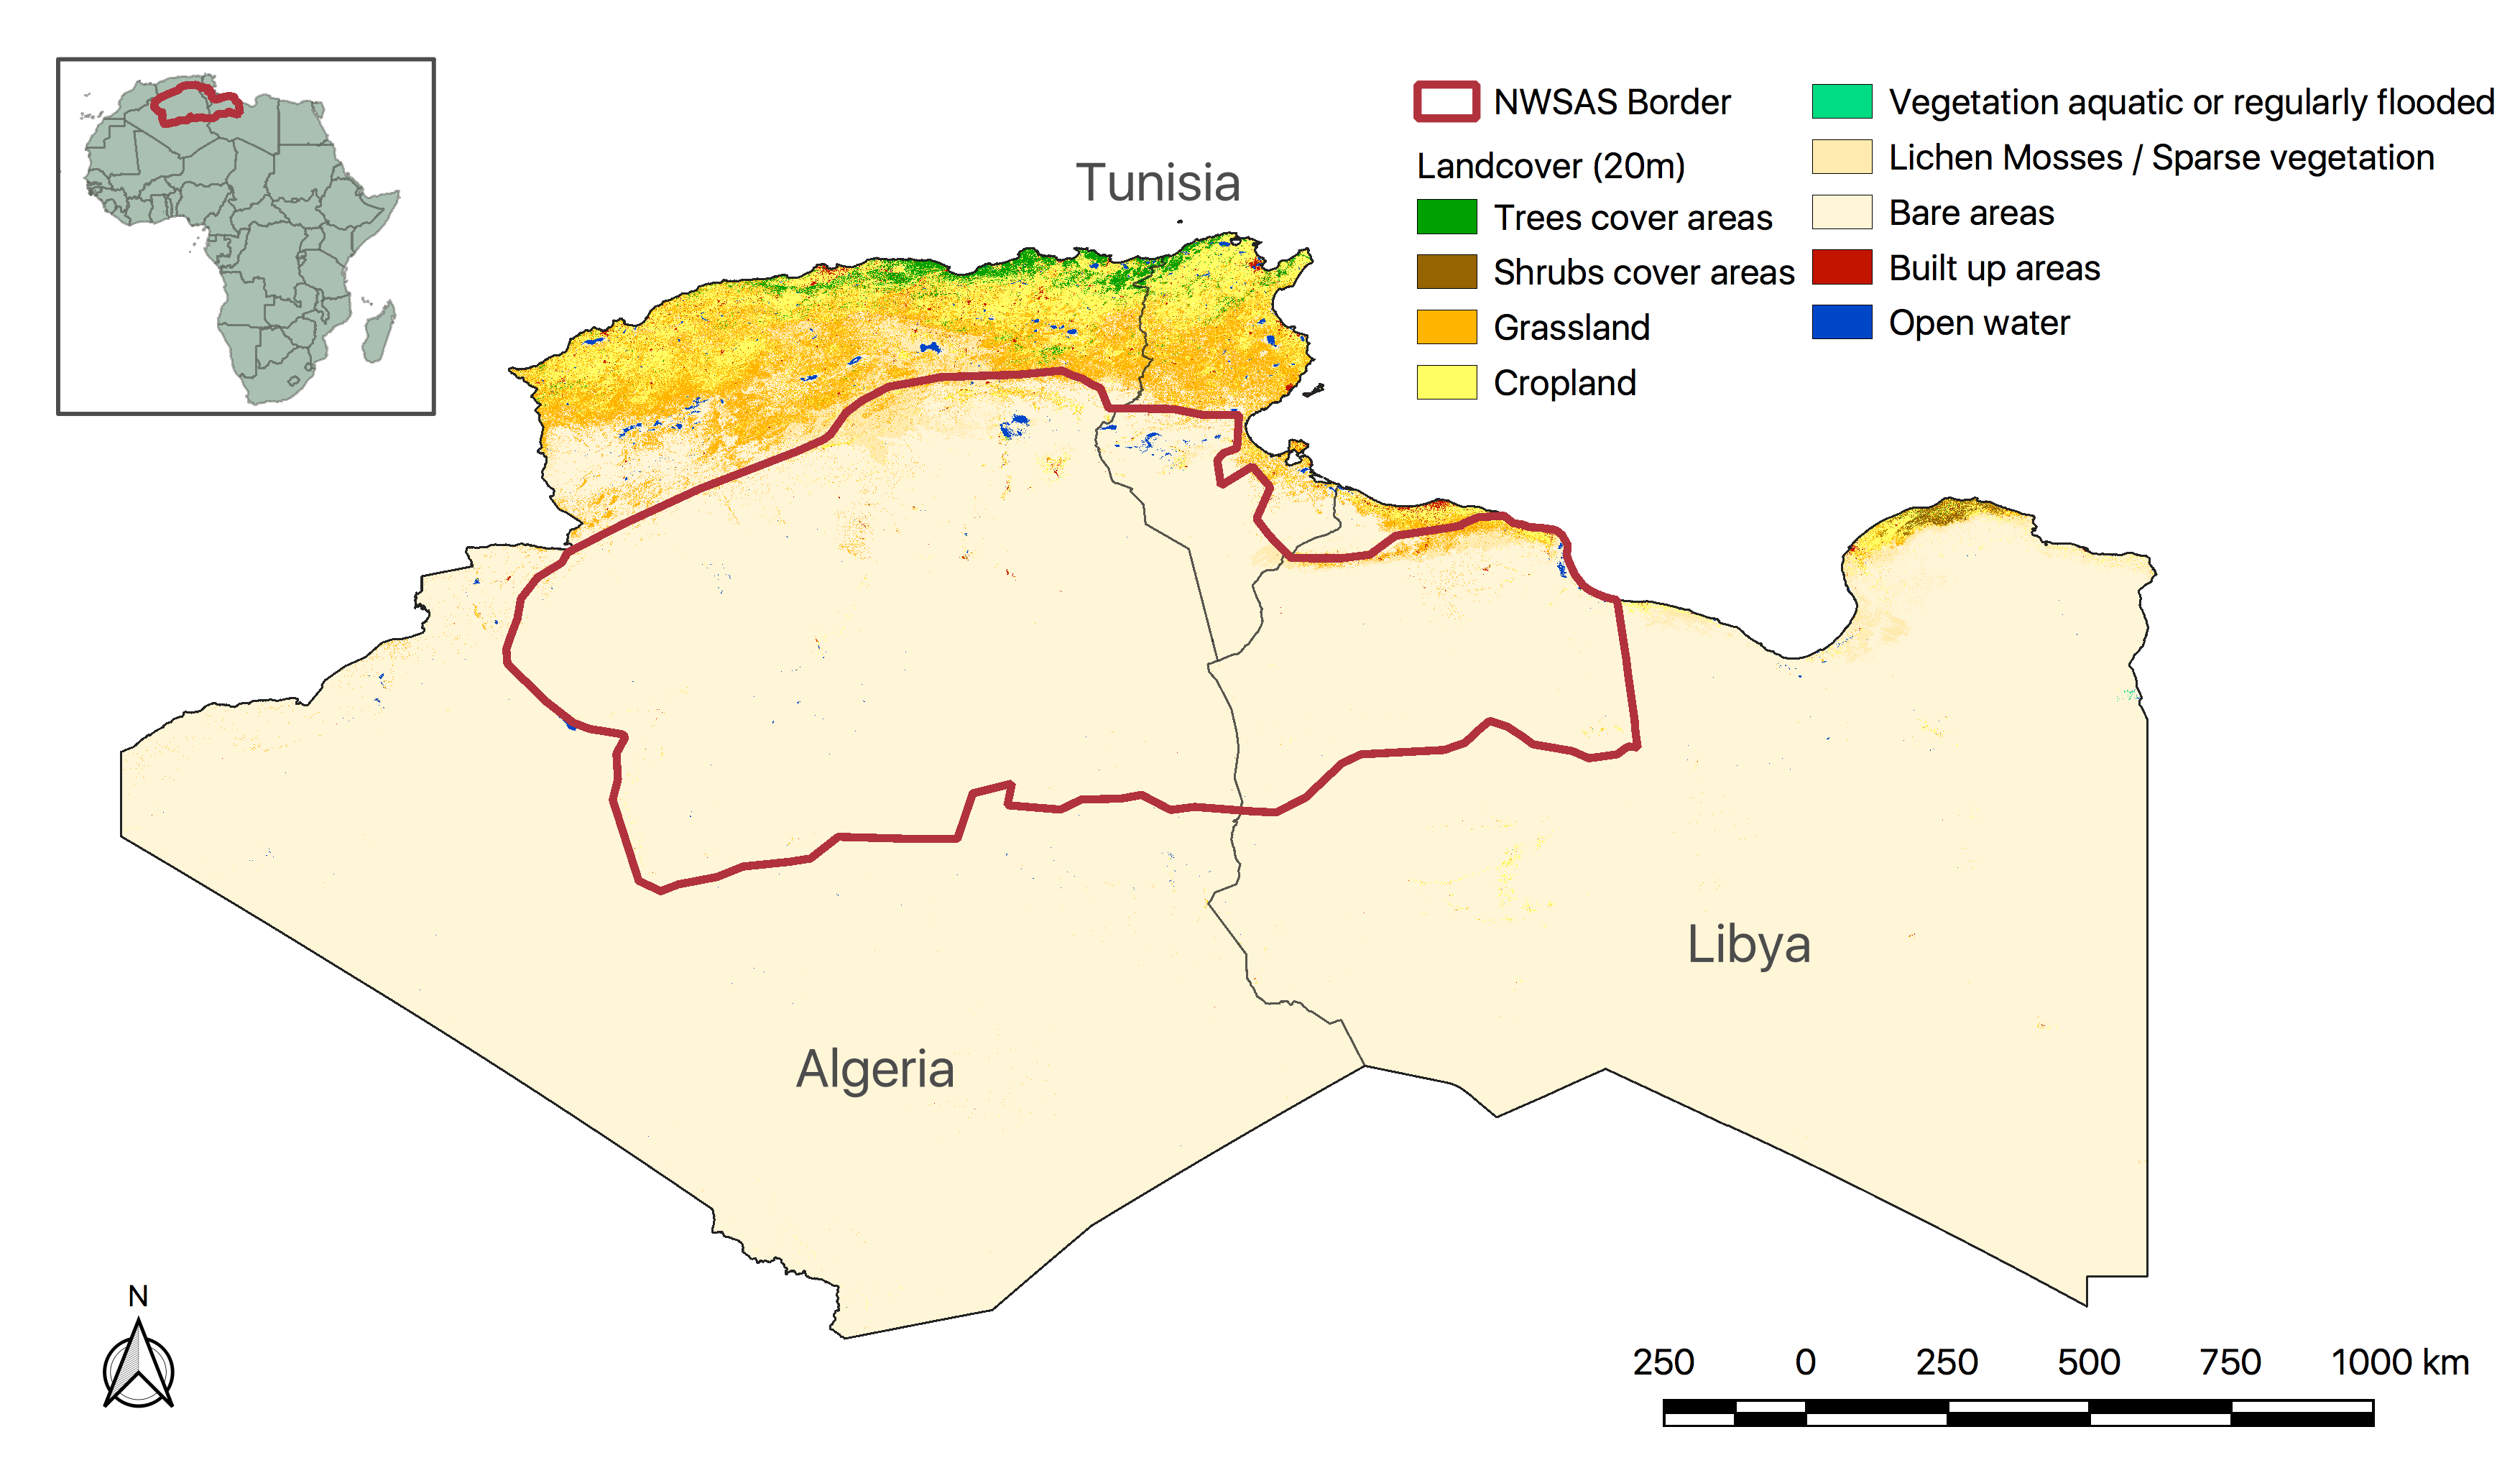
\includegraphics[width=0.9\textwidth]{NWSAS_Landcover}
	\caption[NWSAS land-cover map]{North Western Sahara Aquifer System - Land-cover map at 20$\times$20 meters grid cell resolution.}
	\label{fig:landcover}
\end{figure}

\begin{figure}[!b]
	\centering
	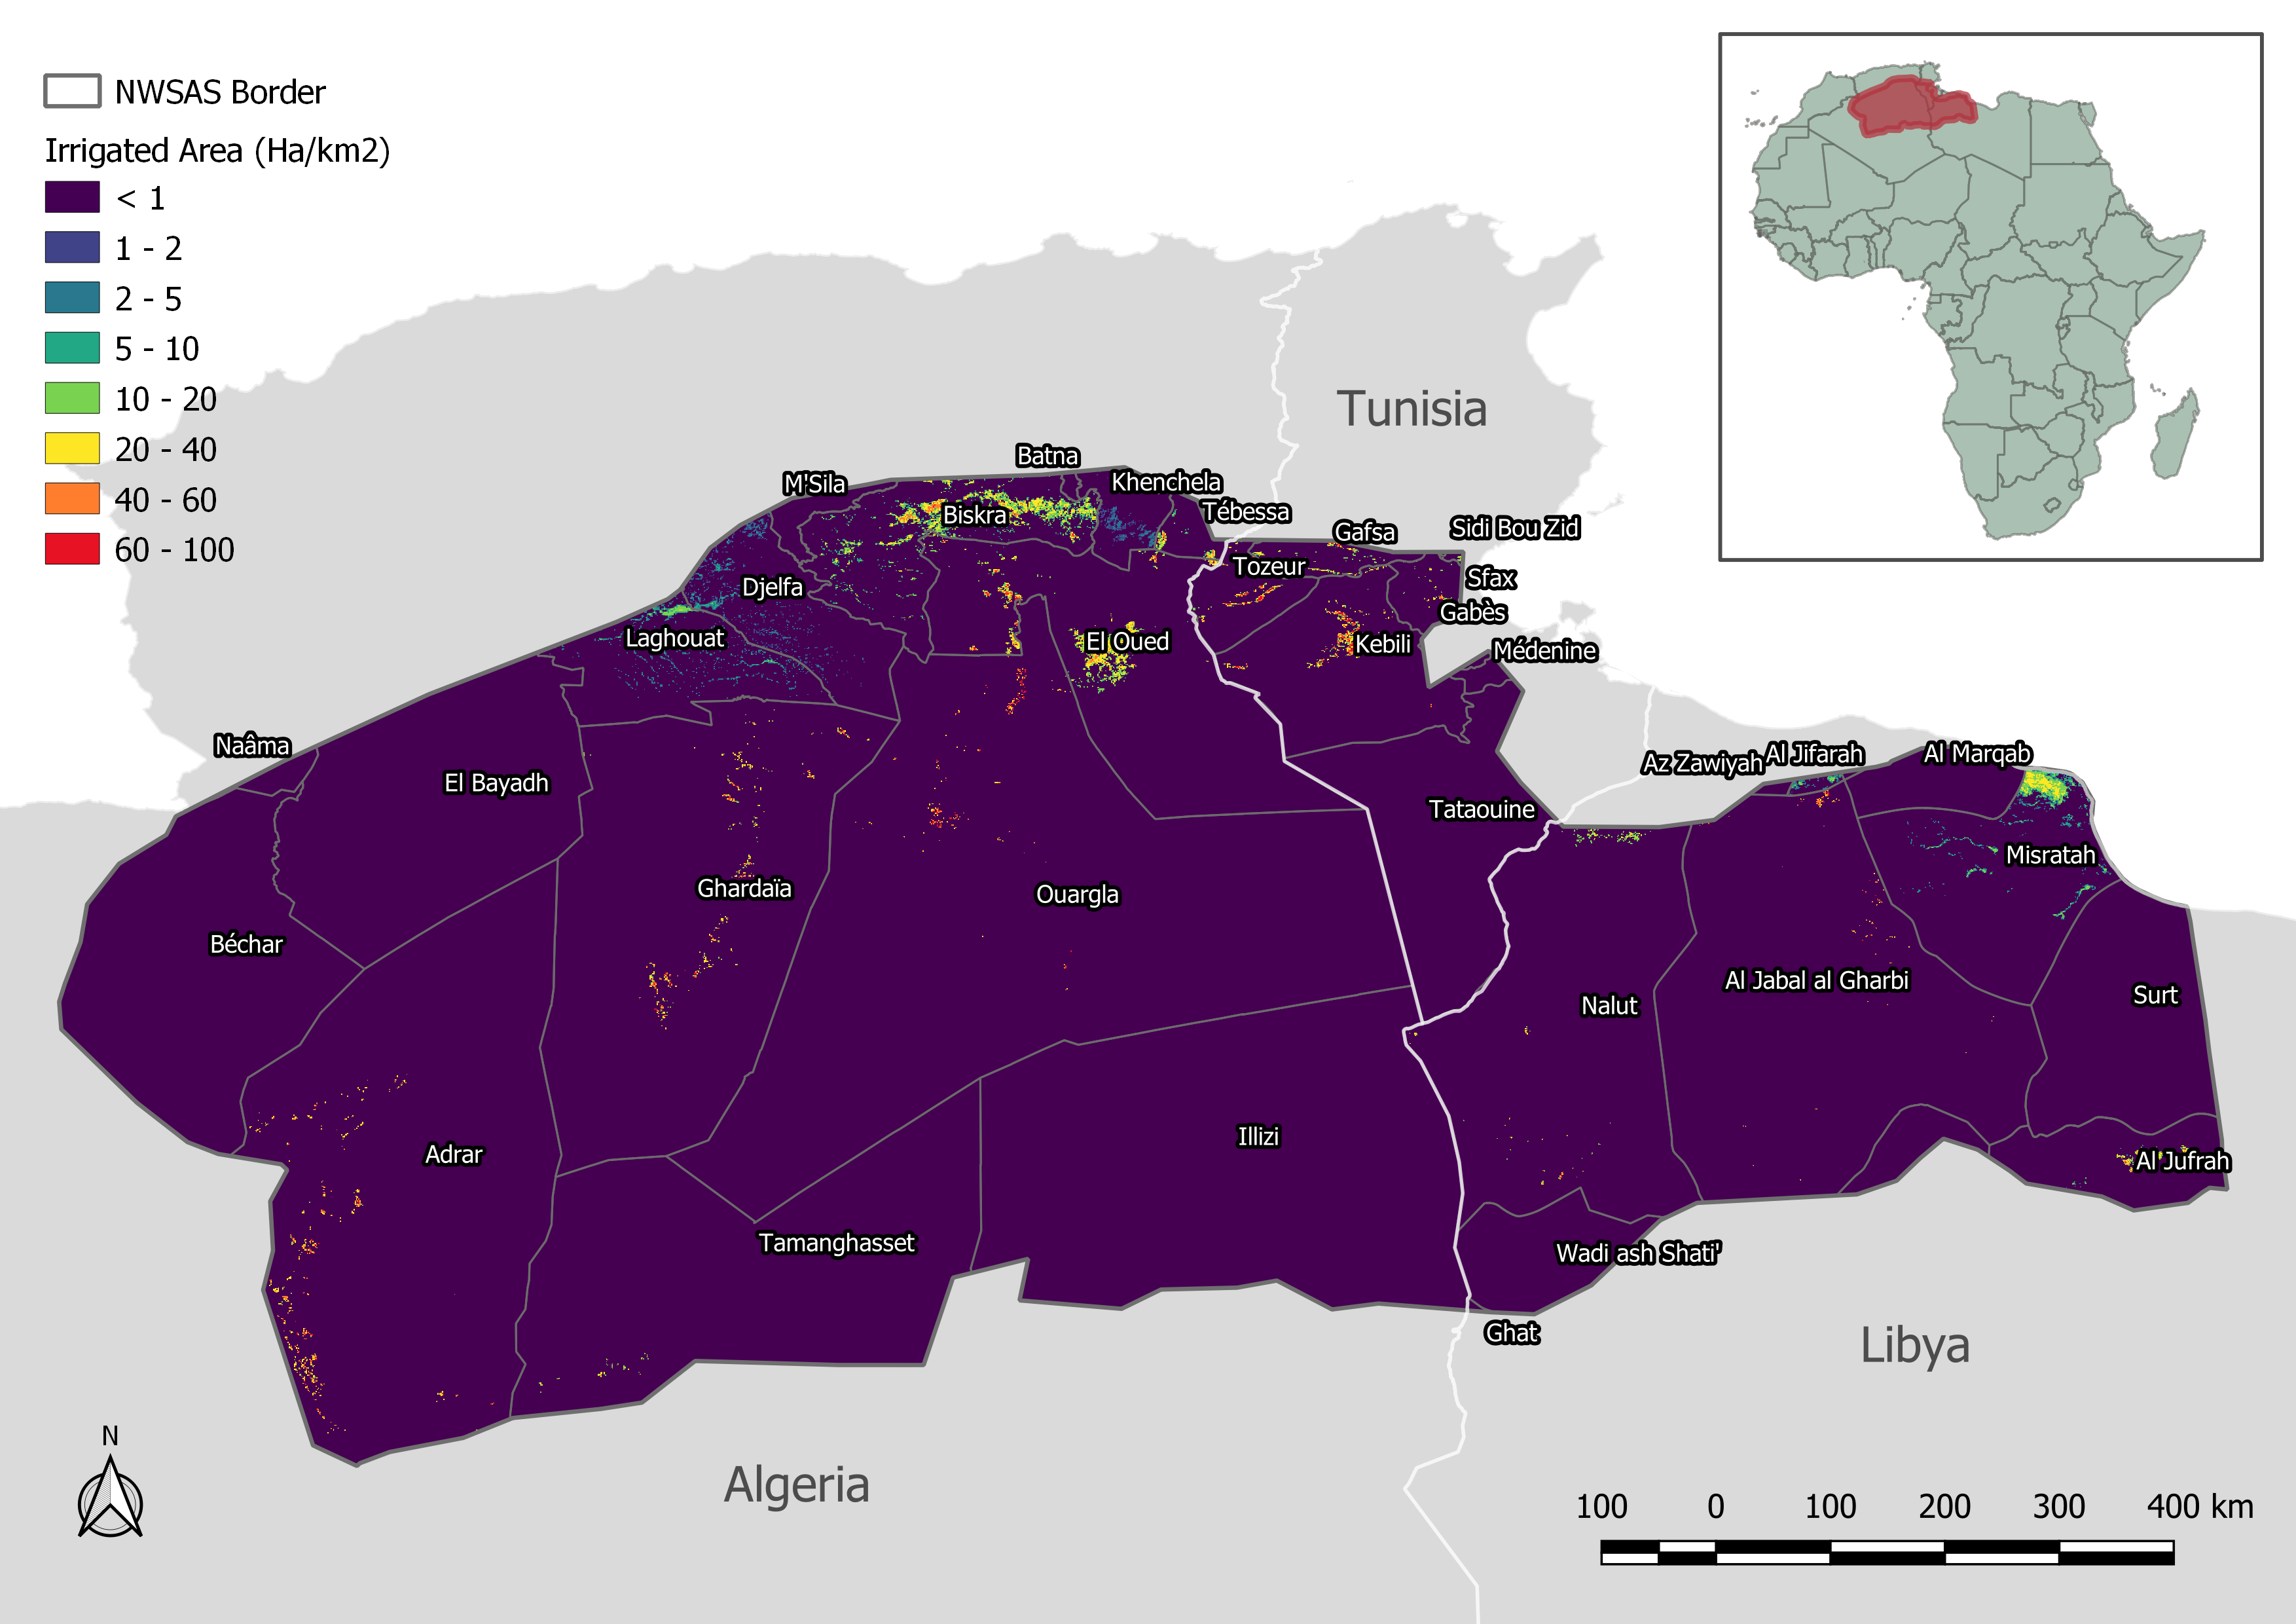
\includegraphics[width=0.88\textwidth, cfbox=black 1pt 0pt]{NWSAS_Irrigated_area}
	\caption[NWSAS cropland density map]{North Western Sahara Aquifer System - Cropland density map at 1$\times$1 km grid cell resolution.}
	\label{fig:irrigated_area}
\end{figure}

From this dataset, some insights can already be obtained. Bare/desertic areas dominate the region, while open water bodies are quite uncommon, however, the water bodies found in the NWSAS region do not constitute ``fresh water" resources due to their high content of salinity \cite{CHAOUKI20131043}. The built up areas are highly scattered throughout the NWSAS region as well as the cropland zones, which are mainly located in the surroundings of the built up areas and in the north of the region. The largest agricultural activity, is given at the north of the three countries, as well as the major urban concentrations, nonetheless, this does not make the NWSAS region less important, as the groundwater resources there, are crucial for ensuring food security for a growing population in the region.

From this land-cover dataset, the cropland areas were subtracted, allowing to create a raster layer containing the cropland density in the region. This layer was created for a resolution of 1km grid cell and calibrated for year 2015 according to regional statistics presented in \autoref{tbl:regionalstats}. The obtained cropland dataset is showcased in \autoref{fig:irrigated_area}.

From \autoref{fig:irrigated_area}, it is depicted with more clarity that the main agricultural activity is in fact, presented in the northern region. The provinces with largest agricultural activity are: Biskra, El Oued, Djelfa, Laghouat, Khenchela, Adrar and Gharda\"\i a in Algeria; Kebili, Tozeur and Gafsa in Tunisia; and Al Marqab, Misratah and Al Jufrah in Libya.

\subsection{Population dataset}
Individual population datasets for Algeria, Tunisia and Libya were obtained from the WorldPop database \cite{Worldpop} in a resolution of 100$\times$100 meters. Afterwards, the three datasets were merged together and masked within the boundaries of the aquifer. The data was then rescaled to a 1 km grid cell resolution and calibrated for year 2015 according to regional statistics (refer to \autoref{tbl:regionalstats}).

\begin{figure}[!ht]
	\centering
	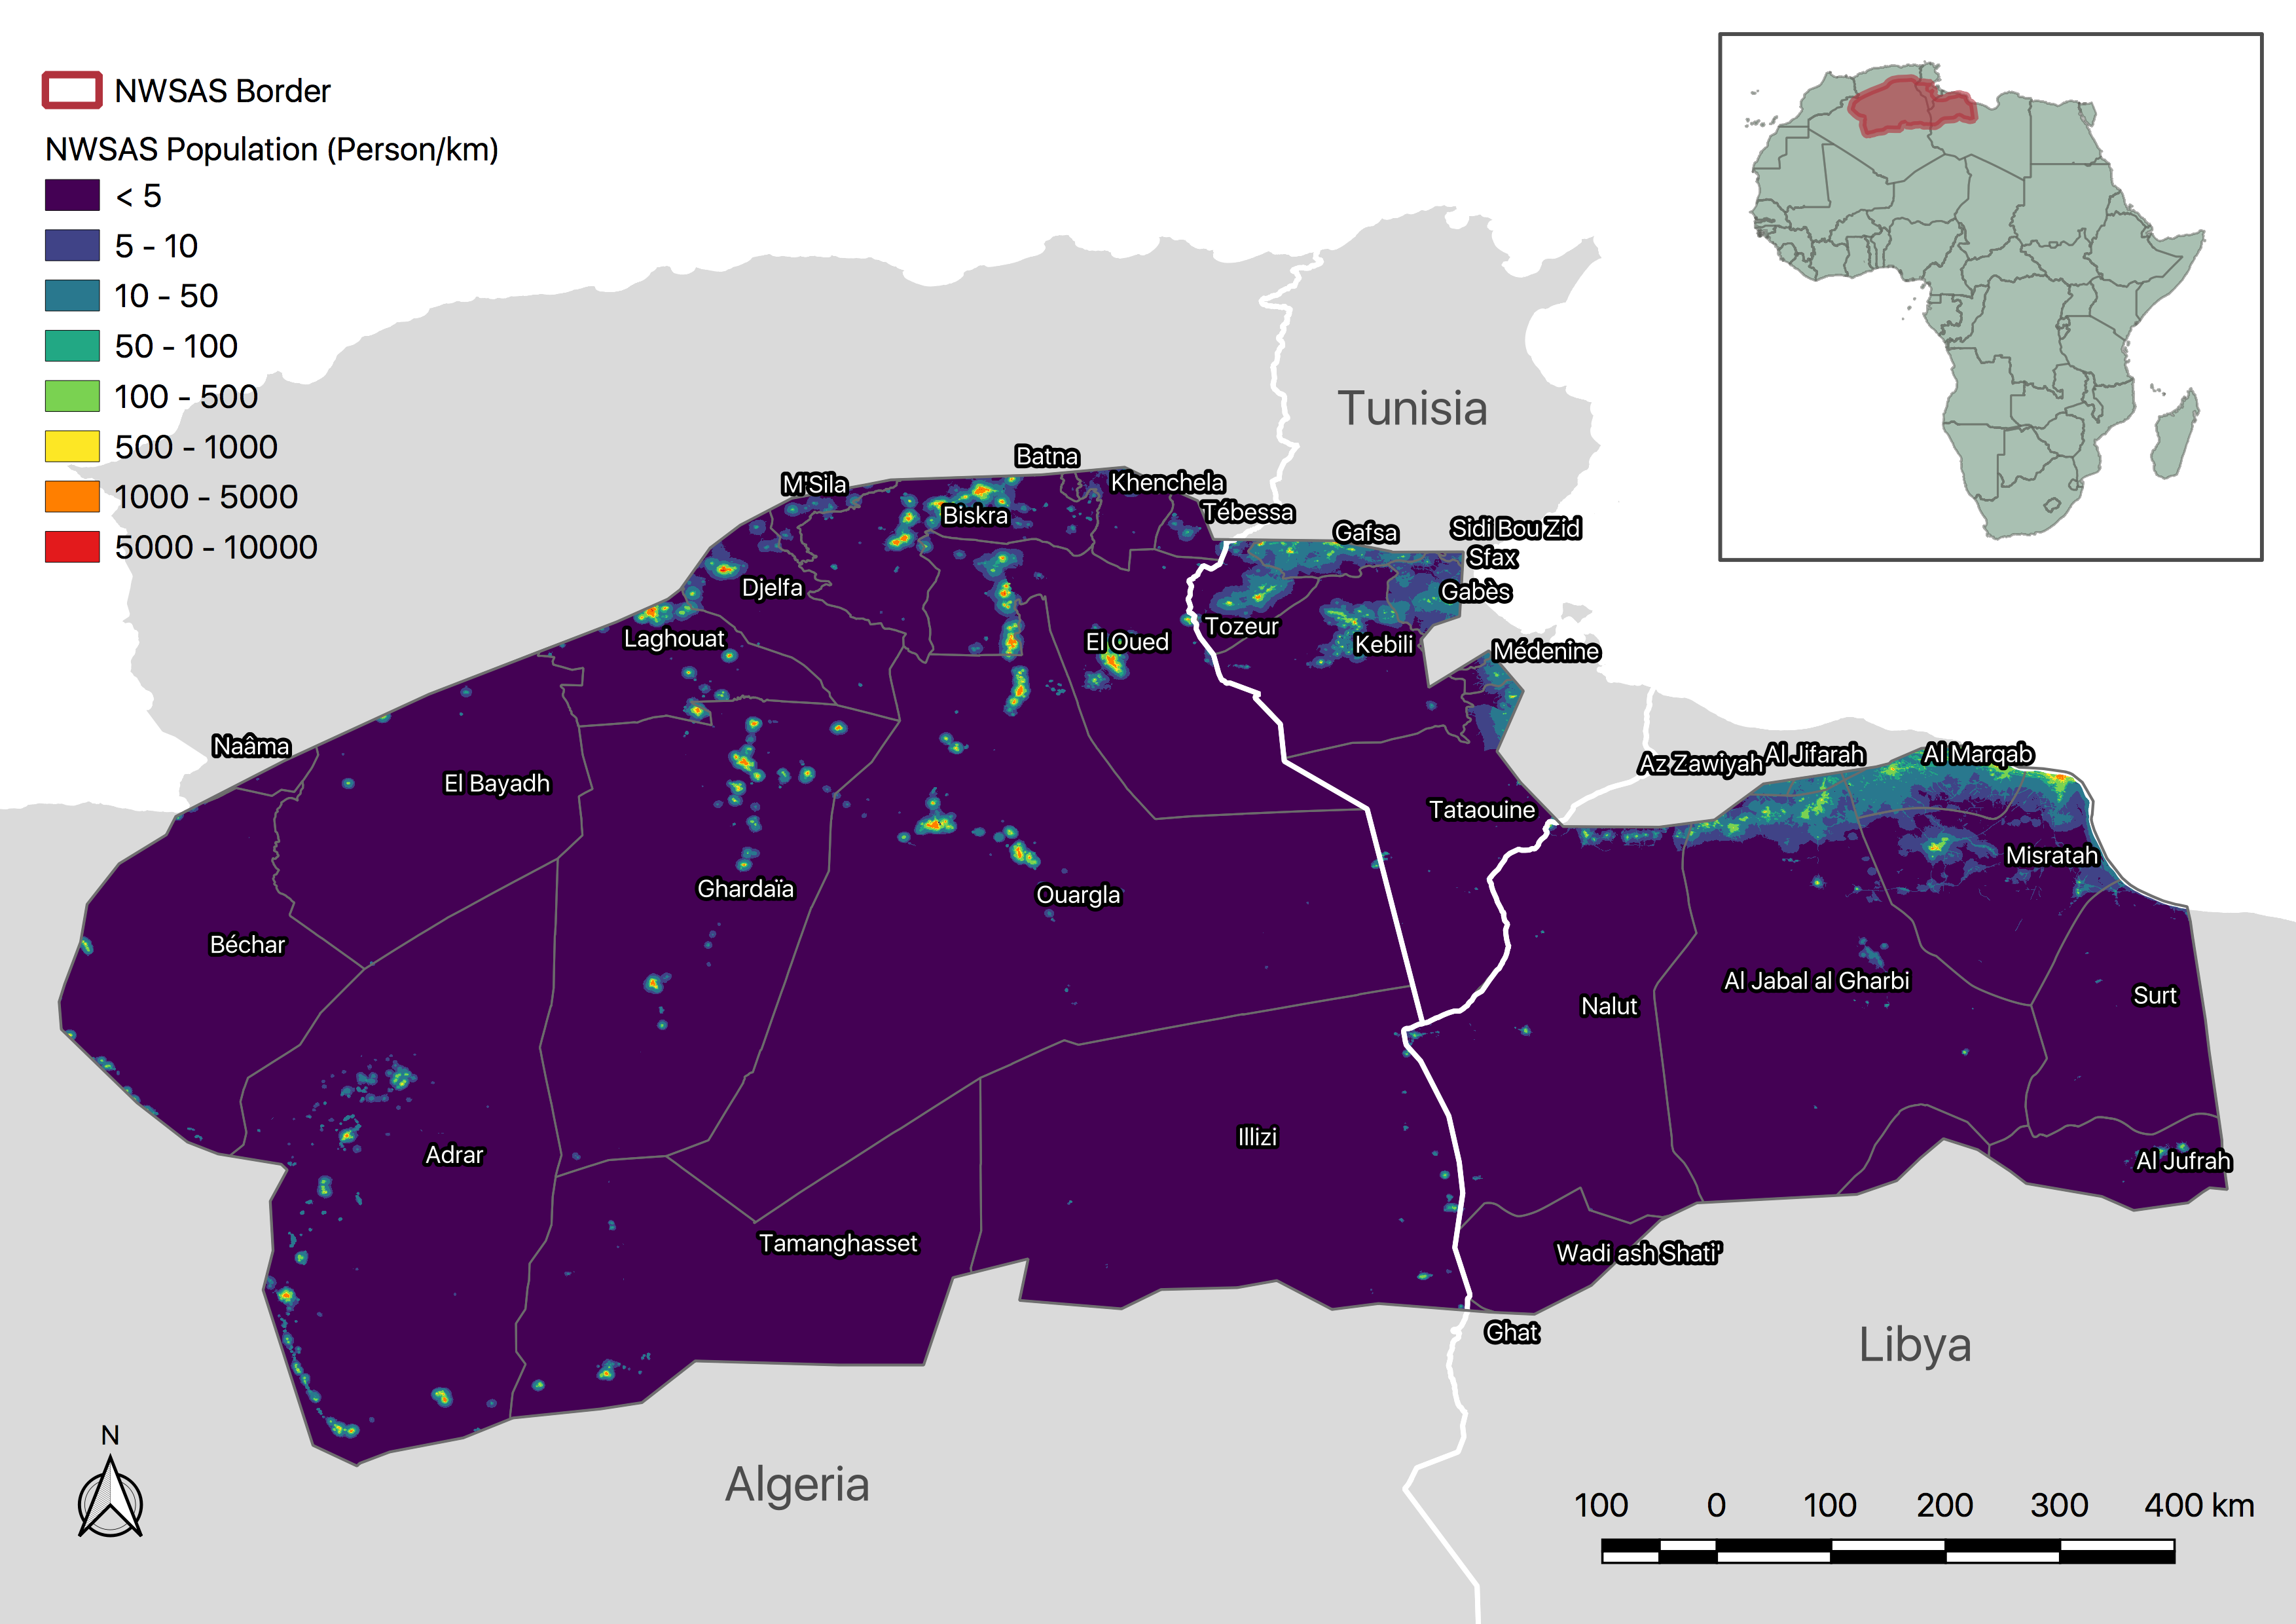
\includegraphics[width=0.88\textwidth, cfbox=black 1pt 0pt]{NWSAS_Population}
	\caption[NWSAS population map]{North Western Sahara Aquifer System - Population density map at 1$\times$1 km grid cell resolution.}
	\label{fig:population}
\end{figure}

\autoref{fig:population} depicts the obtained population layer for the NWSAS region. It is clear that the population agglomerations follow the same location pattern as the cropland areas: scattered through the region with higher concentrations at north of the aquifer. Within Algeria, the provinces with major population count are: Biskra , El Oued, Ouargla, Laghouat, Gharda\"\i a, Adrar and Djelfa. As for Tunisia, Kebili, Tozeur and Gafsa present the higher population counts, although much lower than the Algerian provinces previously mentioned. Moreover, the provinces with higher population count within Libya are Al Marqab, Misratah and Al Jabal al Gharbi.

\subsection{Depth to groundwater dataset}
The depth to groundwater dataset used, was developed by the British Geological Survey for the African continent at a resolution of 5km grid cell. This dataset is underpinned by dedicated case studies and systematic data and literature reviews \cite{Quantitativemapsgroundwater2012a}. The dataset was masked with the NWSAS boundaries and aligned to match the target 1km grid cell resolution (\autoref{fig:depth}).

\begin{figure}[!ht]
	\centering
	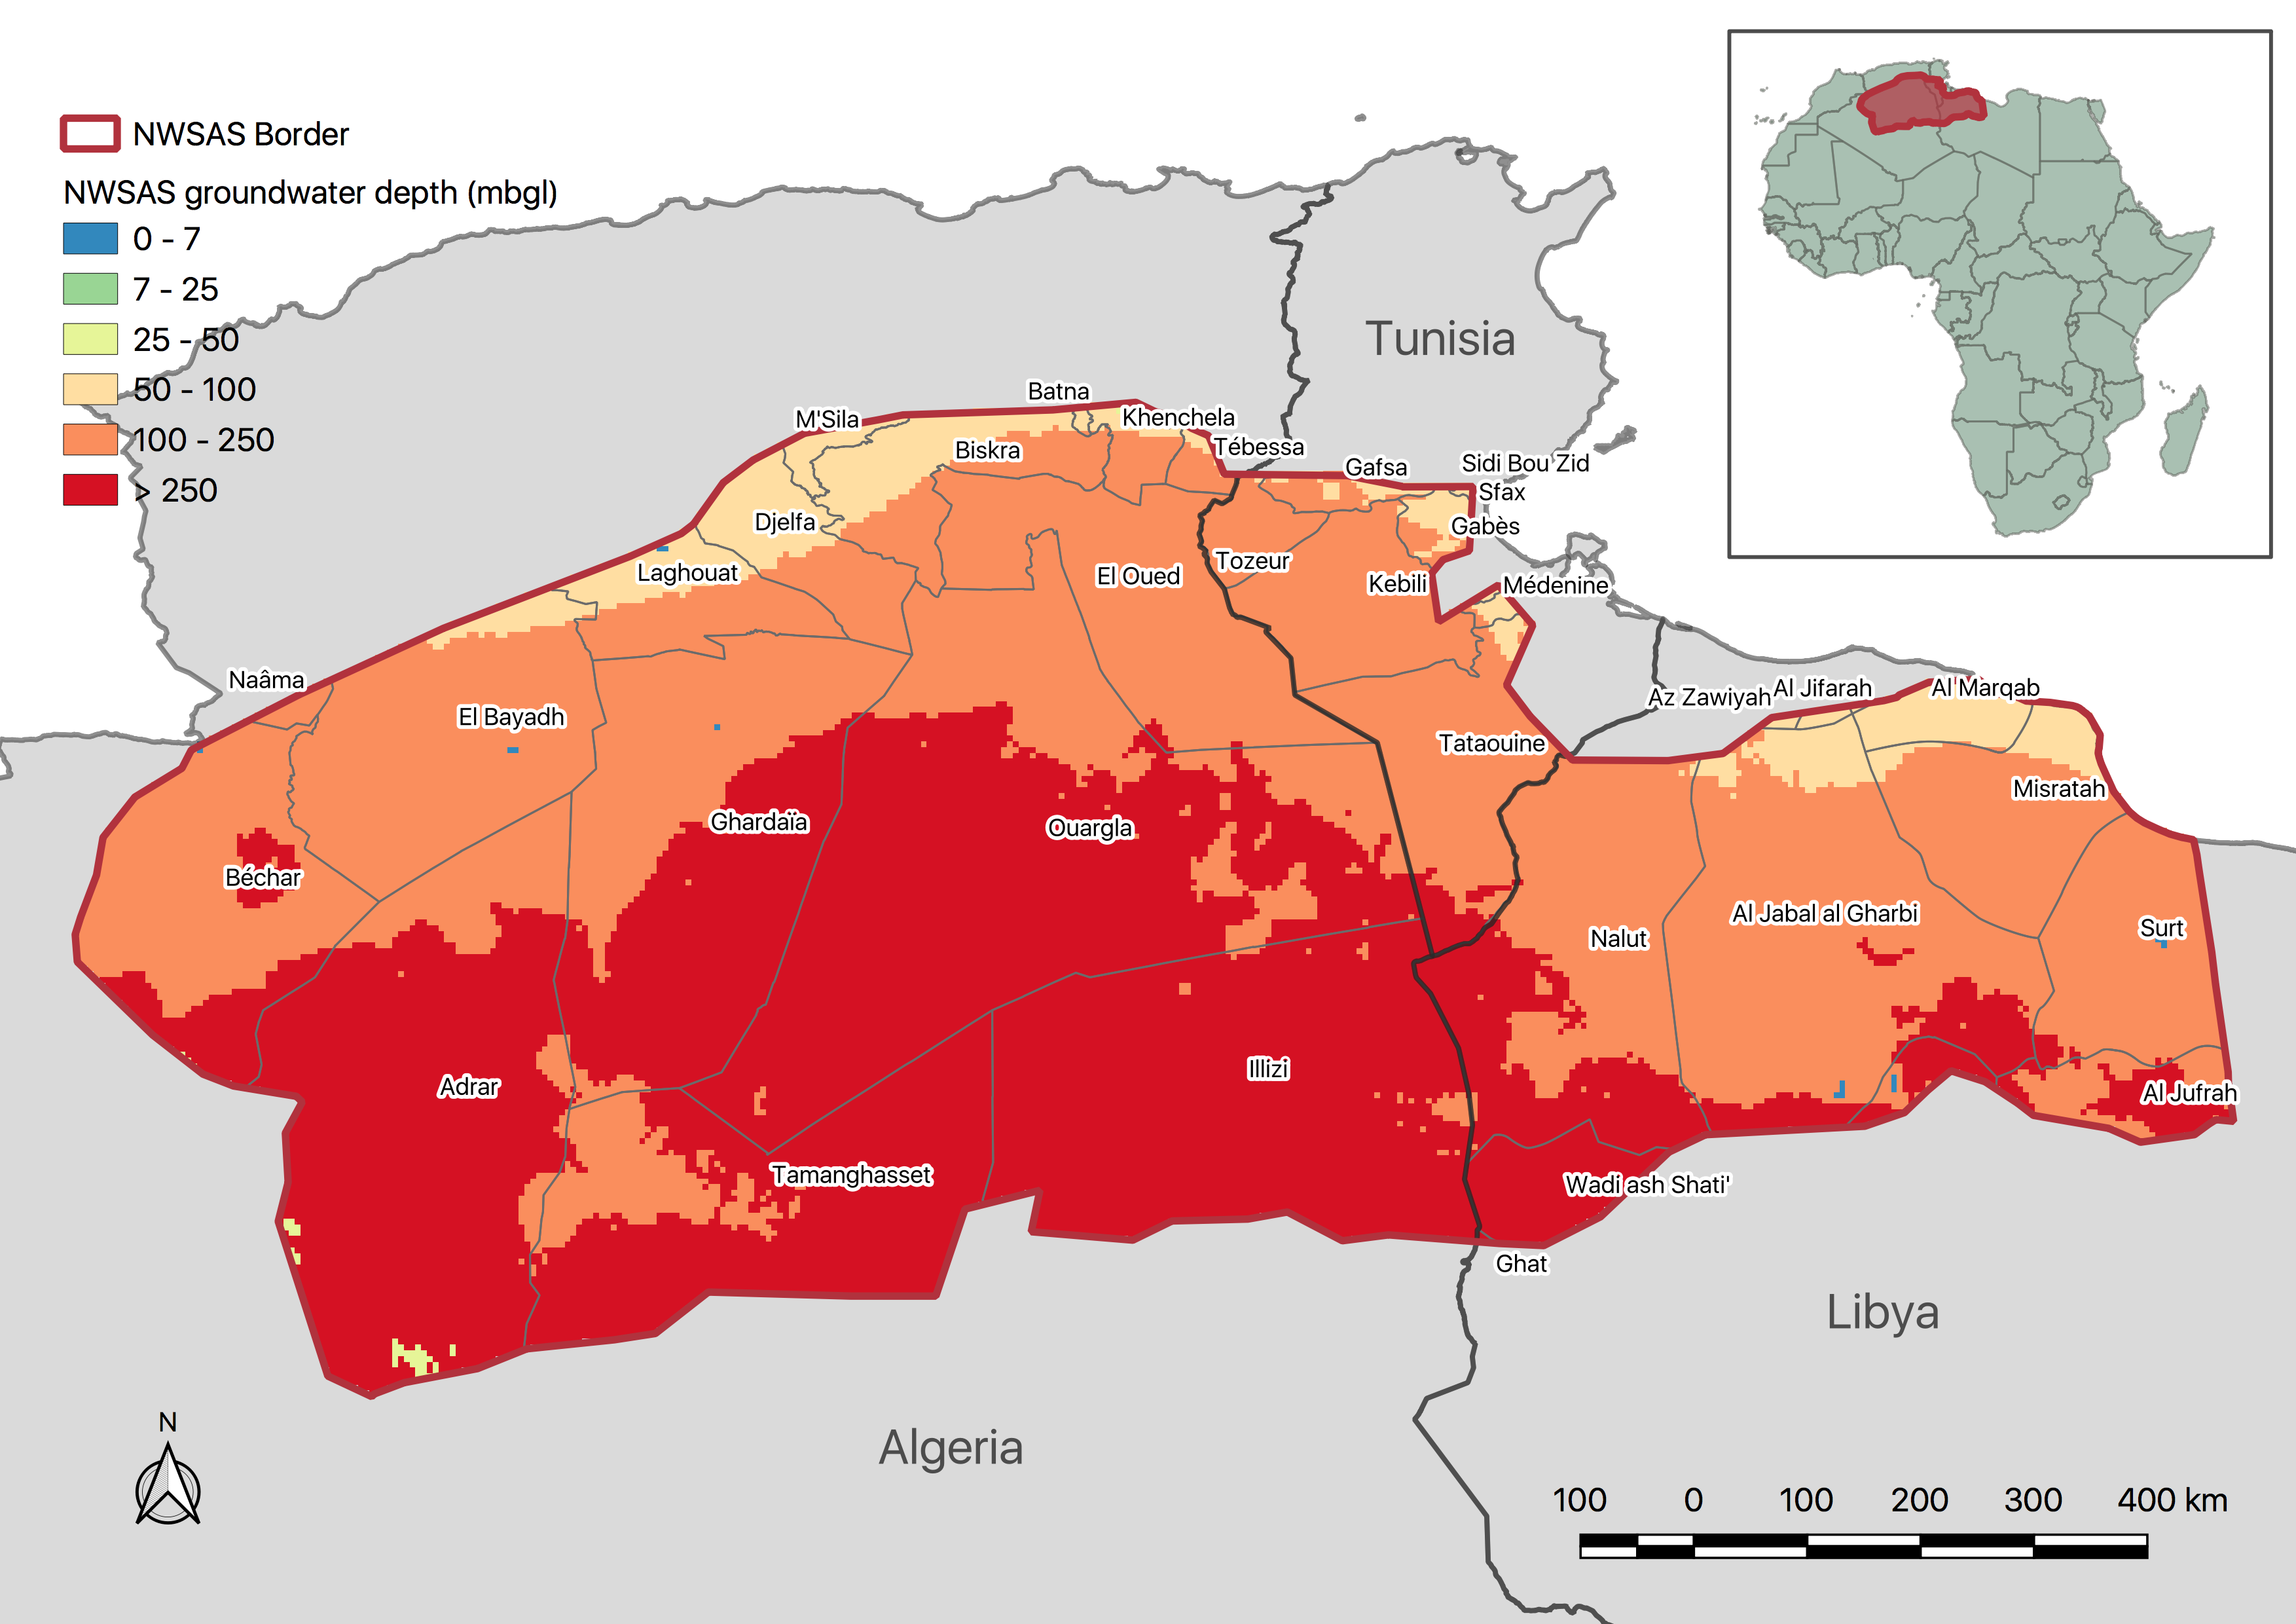
\includegraphics[width=0.88\textwidth, cfbox=black 1pt 0pt]{NWSAS_Depth}
	\caption[NWSAS depth to groundwater map]{North Western Sahara Aquifer System - Depth to groundwater map at 1$\times$1 km grid cell resolution.}
	\label{fig:depth}
\end{figure}

According to this data, it can be seen that the depth to groundwater through the entire aquifer ranges from around 50 to more than 250 meters. In general, in the south of the aquifer the deepest water tables can be found, which could mainly affect the population and agricultural activity of the province of Adrar and part of the provinces of Ouargla and Gharda\"\i a. To the north of the basin, the water table levels decrease to a range between 50 to 100 meters, which can be argued, enables the high agricultural activity there, specially in the province of Biskra.

\section{Data calibration}
The \textit{population} and the \textit{irrigated area} layers were calibrated to match regional statistics. The calibration was performed using the fraction given between the regional statistical data (i.e. total population or total irrigated area), and the sum of all data points of the layer in question. The statistical data was available as per country basis. Thus, the calibration process was performed for the basin areas within each country, using their specific information (see \tref{tbl:regionalstats}).

\begin{table*}[!h]
 \caption{\label{tbl:regionalstats}NWSAS population and irrigated area statistics for year 2015, subdivided per country area inside the basin. Data source: \cite{BetterValorizationIrrigation2015}}
 \begin{indented}
 \item[]\begin{tabular}{@{}l*{4}{r}}
 	\br
 	Parameter & Total & Algeria & Tunisia & Libya\\
 	\mr
 	NWSAS Population & 6,376,367 & 4,240,888 & 617,168 & 1,518,311\\
 	NWSAS Irrigated area (Ha) & 469,529 & 237,485 & 56,547 & 175,497\\
 	\br
 \end{tabular}
 \end{indented}
\end{table*}

Moreover, to calibrate the irrigated area data, an algorithm was run to ensure that non of the data cells had more than 100\% of its area covered by irrigated land.

\section{Population and irrigation water withdrawals}
The calculation of total water withdrawals $ww_{tot,i}$ was performed according to \eref{eq:waterwithdrawals}. Population water withdrawals were calculated as the product between the population count in each data cell ($Pop_{i}$) and the specific water demand per capita ($wpc_{i}$) for the region. Similarly, withdrawals from irrigated agriculture were calculated as the product between the irrigated area inside each data cell ($IrrArea_{i}$) and the specific water demand per cultivated hectare ($wpha_{i}$) for the region.

\begin{equation}\label{eq:waterwithdrawals} 
 ww_{tot,i} = Pop_{i}\cdot wpc_{i} +IrrArea_{i}\cdot wpha_{i} 
\end{equation}

For the baseline, a level of water withdrawals per capita $wpc$ of 55 cubic meters per year was assumed with a population growth of 1\% per year \cite{Householdwaterconsumption2014}. Moreover, all cropland area within the aquifer was considered to be irrigated by groundwater resources and the water requirements per cultivated hectare $wpha$ to be 13,520 m\textsuperscript{3}/Ha for the Algerian part; 13,266 m\textsuperscript{3}/Ha for Tunisia and 9,134 m\textsuperscript{3}/Ha for Libya, according to data from \cite{Socioeconomicaspectsirrigation2014}. Finally, no growth in irrigated area was considered.

\section{Groundwater pumping}\label{Sc:pumping}
The energy needs to pump water from groundwater resources is given by the required lift ($H-h$), the pressure drop due to fluid friction in the piping, and the pressure losses in valves and fittings. Pressure losses due to friction in the piping were found to be rather small compared to the lift requirements. Therefore, and due to lack of specific data on wells and boreholes in the region, the pressure losses due to friction in the piping and in valves and fittings were disregarded. The energy requirements (in watt-h) can then be estimated as \eref{eq:1} \cite{Groundwaterdependentirrigationcosts2017}:

\begin{equation}\label{eq:1}
E = \frac{Q\cdot(\rho\cdot g\cdot(H - h))}{\eta}
\end{equation}

Where $Q$ stands for the water extractions (m\textsuperscript{3}), $\rho$ for the water density (kg/m\textsuperscript{3}), $g$ for the gravitational acceleration (m/s\textsuperscript{2}), $H$ for the delivered hydraulic head (meters), and $h$ for the head in the well (meters). Moreover, $\eta$ accounts for the pumping efficiency, which was set as 85\% along the entire aquifer.

\section{Energy-for-wastewater}\label{Sc:eww}
To calculate the energy-for-wastewater requirements an energy intensity factor was used for each evaluated treatment technology following \eref{eq:energy-for-wastewater}.

\begin{equation}\label{eq:energy-for-wastewater}
E_{ww} = Q_{ww,yr}\cdot X_t
\end{equation}

Where $Q_{ww,yr}$ represents the yearly treated wastewater in m\textsuperscript{3}/yr, and $X_t$ the average energy demand of the specific WWTT $t$, to treat one m\textsuperscript{3} of wastewater (in kWh/m\textsuperscript{3}).

\section{Wastewater Treatment System characteristics}
FAO standards for population wastewater pollutant levels and reused water quality for agricultural irrigation \cite{fao1985water}, were used for the entire NWSAS area. These are shown in \tref{tbl:pollutans}.

\begin{table*}[!ht]
	\caption{\label{tbl:pollutans}Pollutant levels of wastewater and treated wastewater (mg/l).}
	\begin{indented}
	\item[]\begin{tabular}{@{}l r r}
		\br
		Pollutant type & Wastewater & Treated wastewater\\
		\mr
		Suspended solids ($SS$) & 900 & 100\\
		Nitrogen ($N$) & 40 & 10\\
		Phosphorus ($P$) & 20 & 2\\
		Biochemical Oxygen Demand (BOD\textsubscript{5}) ($BOD_5$) & 500 & 50\\
		Chemical Oxygen Demand ($COD$)& 500 & 50\\
		\br
	\end{tabular}
	\end{indented}
\end{table*}

Cost functions for different WWTT taken from the work of \citet{Assessmentwastewatertreatment2012}, were used to evaluate the competence of selected technologies in the NWSAS. Energy intensity characteristics were added for each technology according to \cite{Energypatternanalysis2012,ComparativeAnalysisEnergy2017}. The characteristics of the different WWTT and their cost and energy functions are presented in \tref{tbl:treatmentsystems}.

\begin{table*}[!h]
    \caption{\label{tbl:treatmentsystems}Treatment systems analyzed Adapted from \cite{Assessmentwastewatertreatment2012}, Copyright (2012), with permission from Elsevier.}
    \addtocounter{table}{-1}
\end{table*}
	~\\[-50pt]{\footnotesize
	\begin{longtable}{@{}P{1.2in} P{0.9in} P{1.9in} P{0.7in} P{0.7in}}
	\br
    Technology & Pollutant removal (\%) & Costs (\euro) & Energy (kWh)$^{\dagger}$ & Usage\\
    \mr
    \endfirsthead
    \multicolumn{4}{@{}l}{\ldots continued}\\\br
    Technology & Pollutant removal (\%) & Costs (\euro) & Energy (kWh)$^{\dagger}$ & Usage\\\mr
    \endhead % all the lines above this will be repeated on every page
    \br
    \multicolumn{4}{r@{}}{continued \ldots}\\
    \endfoot
    \endlastfoot
    Pond System (PS) & N: 20 -- 40 \newline P: 60 -- 70 \newline COD: 60 -- 96 \newline SS: 50 -- 90 & CAPEX: $3897.7\cdot x^{-0.407}$ \newline OPEX: $5.543\cdot x + 3127.5$ & $0.19\cdot V$ & Irrigation tailwater\\
    Intermittent Sand Filter (ISF) & N: 65 -- 95 \newline P: 75 -- 99 \newline COD: 75 -- 90 \newline SS: 85 -- 95 & CAPEX: $2115.5\cdot x^{-0.399}$ \newline OPEX: $12.026\cdot x+3518.9$ & $0.2\cdot V$ & Domestic wastewater\\
    Trickling Filter (TF) & N: 35 -- 50 \newline P: 35 -- 55 \newline COD: 75 -- 90 \newline SS: 50 -- 90 & CAPEX: $12237\cdot x^{-0.87}$ \newline OPEX: $13.504\cdot x+6020$ & $0.3\cdot V$ & Domestic wastewater\\
    Moving Bed Biofilm Reactor (MBBR) & N: 10 -- 20 \newline P: 30 -- 40 \newline COD: 20 -- 40 \newline SS: 60 -- 80 & CAPEX: $1187\cdot x^{-0.165}$ \newline OPEX: $12.794\cdot x+6031$ & $0.8\cdot V$ & Domestic wastewater\\
    Rotating Biological Contractors (RBC) & N: 20 -- 80 \newline P: 10 -- 30 \newline COD: 70 -- 93 \newline SS: 75 -- 98 & CAPEX: $6931.4\cdot x^{-0.383}$ \newline OPEX: $313.4\cdot x^{-0.435}$ & $0.8\cdot V$ & Domestic wastewater\\
    Membrane Bioreactor (MBR) & N: 50 -- 90 \newline P: 20 -- 70 \newline COD: 70 -- 90 \newline SS: 85 -- 99 & CAPEX: $5635.3\cdot x^{-0.352}$\newline $^{*}$OPEX: $2.116\cdot V^{0.713}e^{1.51\cdot SS+0.037\cdot BOD}$ & $0.8\cdot V$ & Domestic wastewater\\
    Extended Aeration (EA) & N: 50 -- 90 \newline P: 15 -- 70 \newline COD: 70 -- 90 \newline SS: 85 -- 99 & CAPEX: $7946\cdot x^{-0.460}$ \newline $^{*}$OPEX: $169.48\cdot V^{0.454}e^{0.61\cdot SS}$ & $0.6\cdot V$ & Domestic wastewater\\
    Sequencing Batch Reactor (SBR) & N: 55 -- 90 \newline P: 25 -- 70 \newline COD: 70 -- 90 \newline SS: 85 -- 99 & CAPEX: $8258.9\cdot x^{-0.407}$ \newline OPEX: $309.4\cdot x^{-0.389}$ & $1\cdot V$ & Domestic wastewater\\
    \br
    \multicolumn{4}{@{}l}{$x$: population equivalent, $x=V\times1500/(400\times365)$, $V$: wastewater flow (m\textsuperscript{3}/yr)} \\
    \multicolumn{4}{@{}l}{N: Nitrogen, P: Phosphorus, COD: Chemical Oxygen Demand, SS: Suspended Solids} \\
    \multicolumn{4}{@{}l}{CAPEX: Capital Expenditure, OPEX: Operating Expenses}\\
    $^{*}$ Taken from \cite{Costmodellingwastewater2011} & & & \\ 
    $^{\dagger}$ Based on \cite{Energyrequirementswater2012,ComparativeAnalysisEnergy2017} & & & 
    \end{longtable}
	}

\section{Reverse Osmosis desalination}\label{Sc:RO}
Reverse Osmosis (RO) desalination is the most popular desalination technology used worldwide. Its energy intensity falls typically in the range of 0.5 to 2.5 kWh per cubic meter of desalinated brackish water \cite{Energyoptimalgroundwater2013}.

To estimate the energy required to desalinate one cubic meter of saline water, often detailed information of the RO system is required. When analysing a broad area using a geospatial approach, such information is not available as the characteristics of the system can change from application to application \cite{stillwellPredictingSpecificEnergy2016,aminfardMultilayeredSpatialMethodology2019}. Thus, a simplified approach was used to estimate the RO energy requirements. RO is a pressure-driven process that forces water through a membrane which separates dissolved solutes using preferential diffusion. The output water from the membrane (\textit{permeate, p}) is relatively free of solutes, while the remaining water (\textit{concentrate, c}) exits the pressure vessel with a high concentration of solutes (i.e. high TDS levels). A schematic representation of the process is presented in \fref{fig:ro} \cite{crittenden_mwhs_2012}.

\begin{figure}[!h]
	\centering
	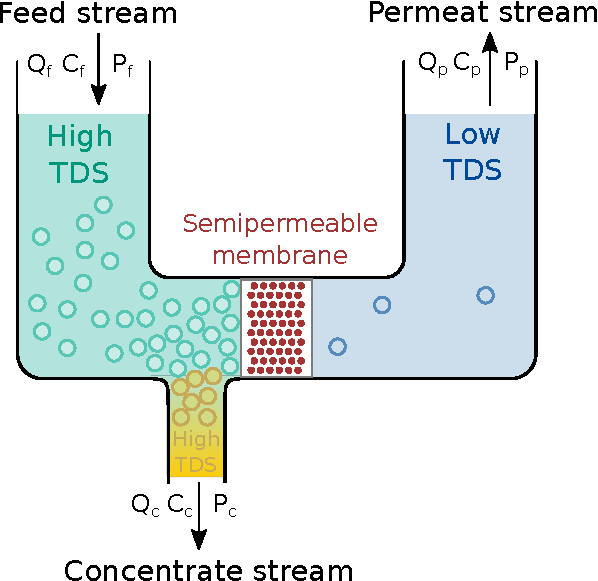
\includegraphics[width=0.4\textwidth]{Reverse_Osmosis}
	\caption[Reverse Osmosis schematic separation process]{Reverse osmosis schematic separation process. Based on: \cite{crittenden_mwhs_2012}.}
	\label{fig:ro}
\end{figure} 

The minimum energy required to push the water through the membrane is given by the amount of diluted solutes in the \textit{feed (f)} water. Such minimum energy can be estimated calculating the osmotic pressure of the \textit{feed} water, as described in \eref{eq:6} \cite{crittenden_mwhs_2012}.

\begin{equation}\label{eq:6}
\pi = \phi\cdot C\cdot R\cdot T
\end{equation}

\noindent{Where}:
\begin{itemize}[label={-}]
	\item $\pi$: osmotic pressure (bar),
	\item $\phi$: osmotic coefficient, close to 1 (-), assumed a 0.95 \cite{crittenden_mwhs_2012},
	\item $C$: concentration of all solutes (mol/L),
	\item $R$: universal gas constant, 0.083145 (L$\cdot$bar/mol$\cdot$K),
	\item $T$: absolute temperature (K), (273 + \degree C), assumed at 25 \degree C for the entire aquifer.
\end{itemize}~

Thus, the minimum energy demand can be estimated multiplying the osmotic pressure of the \textit{feed} water $\pi$ (in bar) by a conversion factor of 1.0 kWh/m\textsuperscript{3} = 36 bar. In reality, the energy demanded is greater due to factors as friction losses, membrane filtration resistance, among others. However, this approach has been used in cases were no specific data of the RO system is available \cite{KARABELAS201815}.

\begin{figure*}[!h]
	\centering
	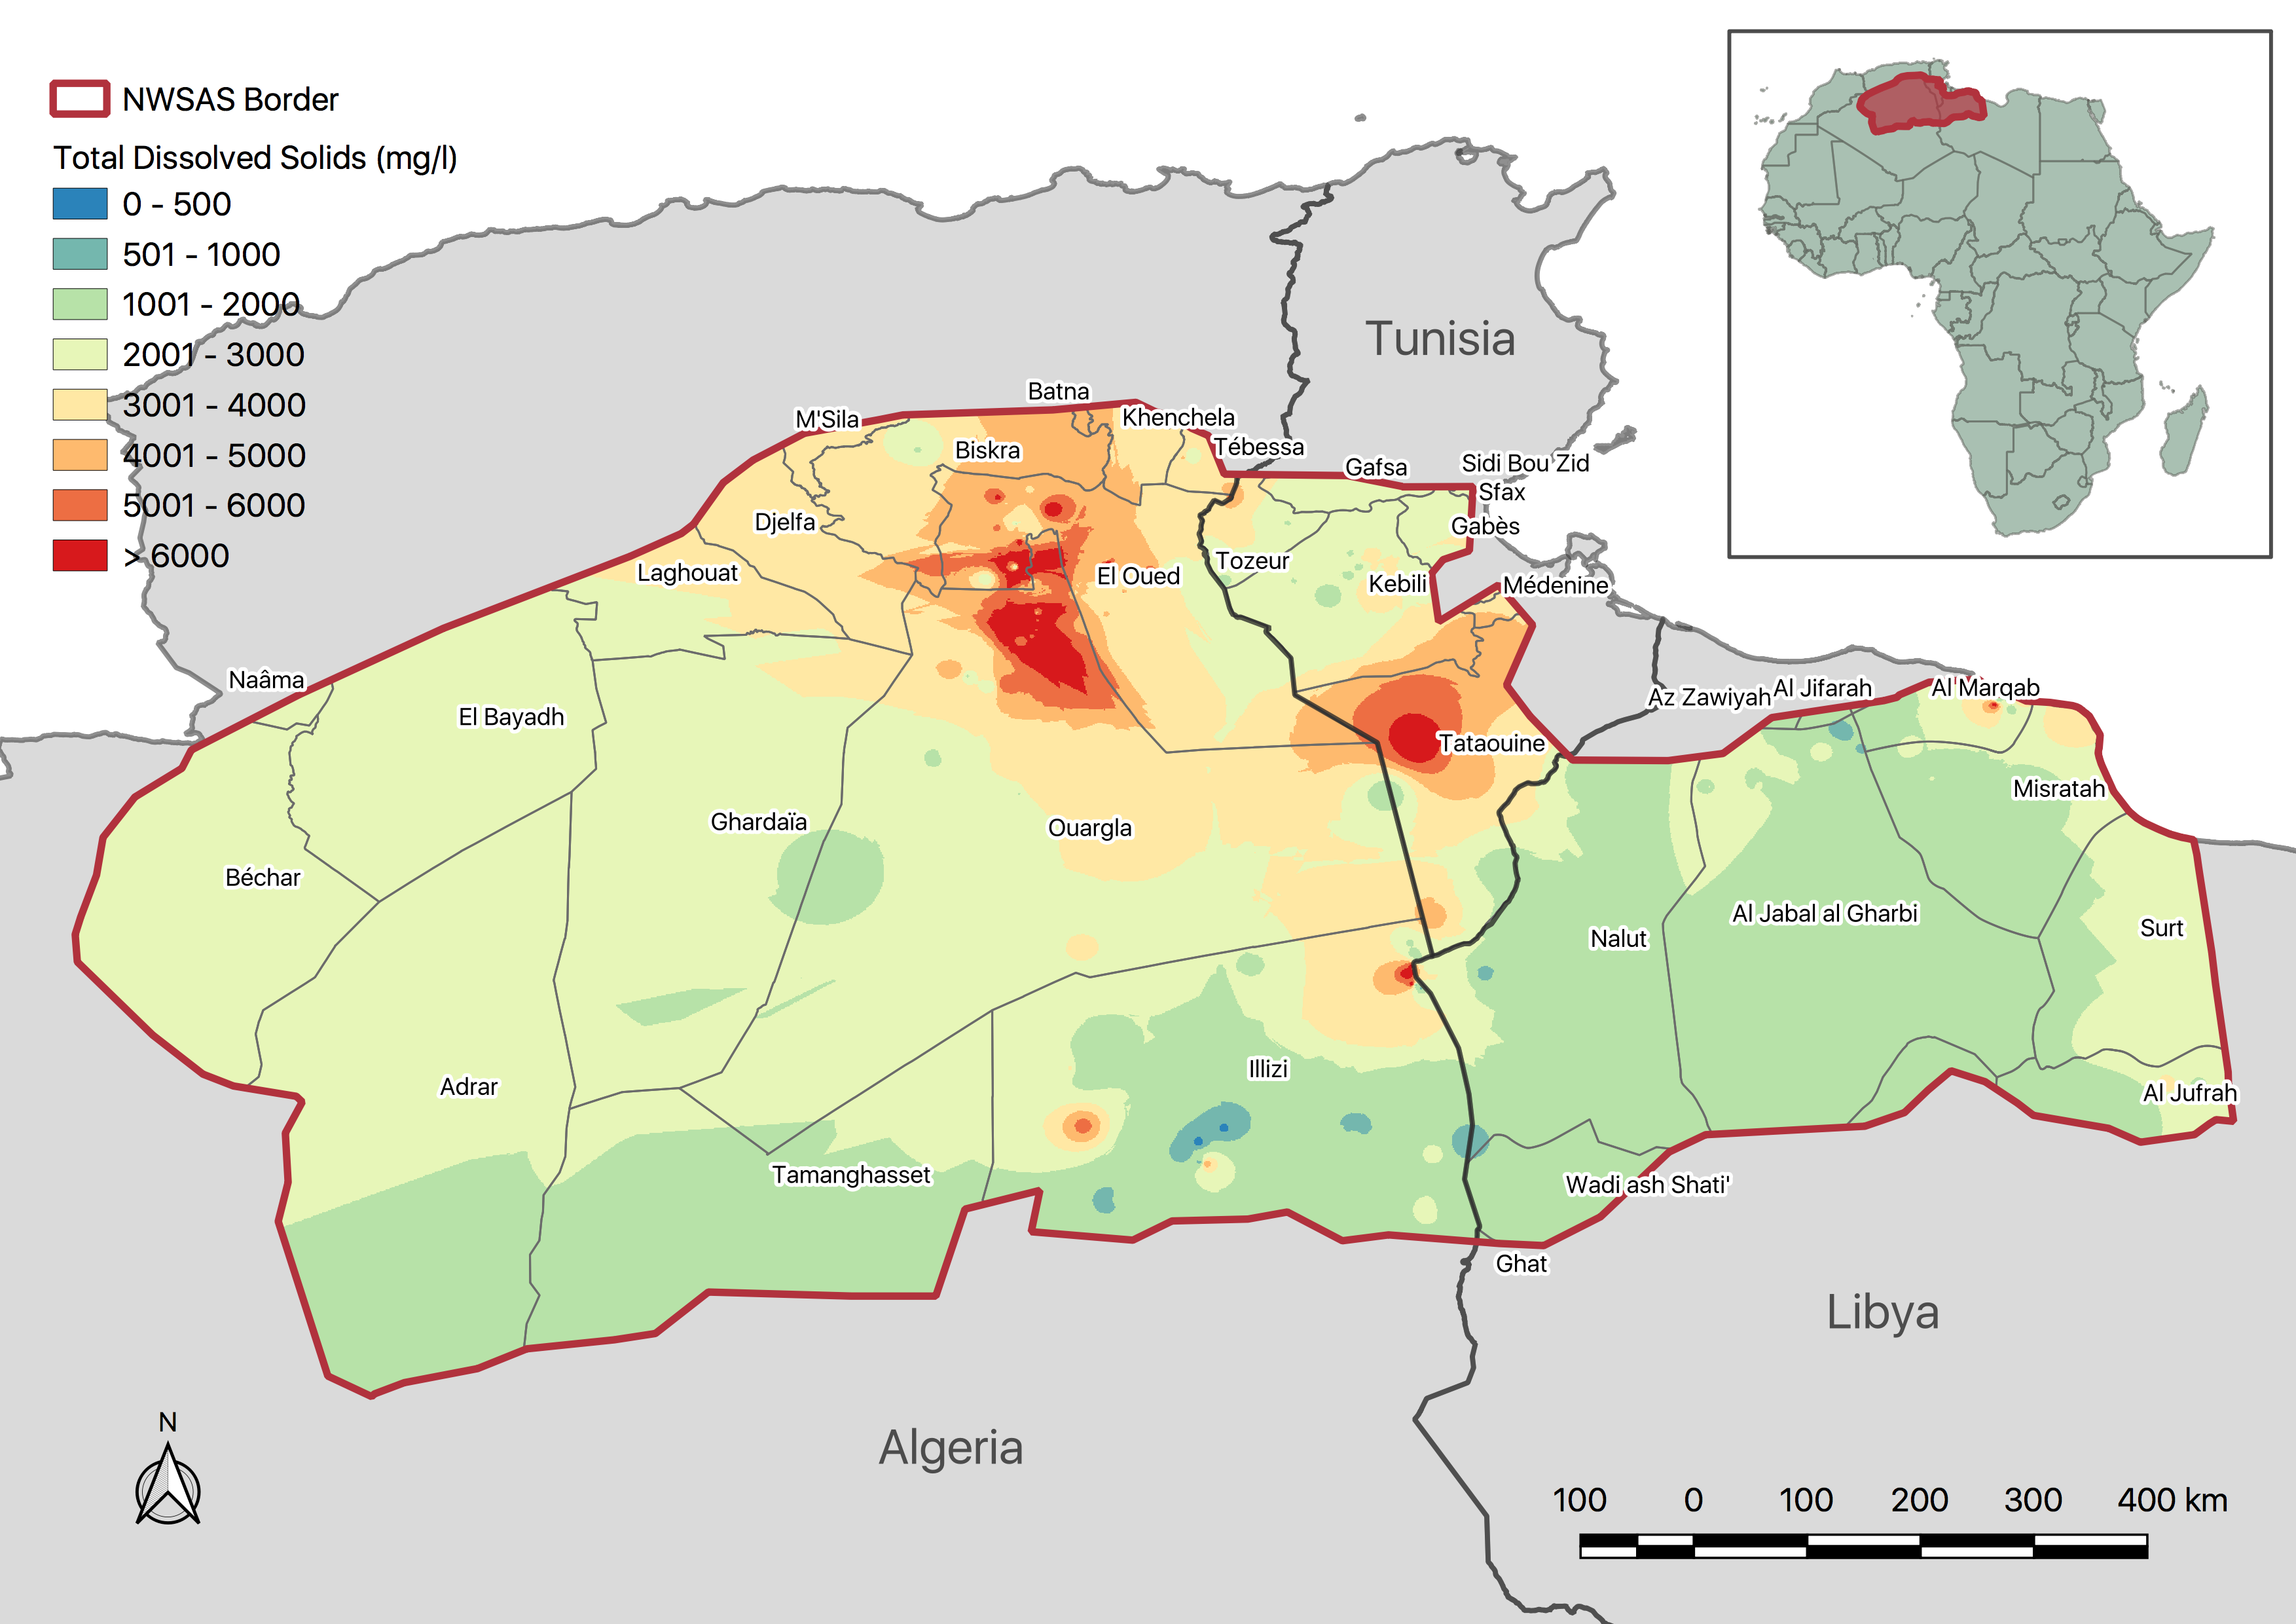
\includegraphics[width=0.88\textwidth, cfbox=black 1pt 0pt]{NWSAS_TDS}
	\caption[NWSAS groundwater quality map - Total Dissolved Solids (TDS)]{North Western Sahara Aquifer System - Groundwater quality map, Total Dissolved Solids (TDS) at 1$\times$1 km grid cell resolution.}
	\label{fig:TDS}
\end{figure*}

The water quality layer used, was obtained from 206 measurements provided by National Authorities of the region. Each point specifies the spacial location and groundwater TDS content. Although the data did not covered the entire basin area, due to lack of any other related information it was used to produced a raster layer. An inverse distance weighted interpolation method, having as distance weighting factor an inverse distance to a power of 2 and a global search radius with maximum number of nearest points of 10 was used (see \fref{fig:TDS}).

\section{Levelised Cost of Water (LCOW)}
\autoref{eq:lcow}, disaggregates the $LCOW$ (\$/m\textsuperscript{3}) value in three components: the cost components due to investment $LCOW_{Inv}$, operation and maintenance $LCOW_{O\&M}$ and externalities $LCOW_{Ext}$.

\begin{equation}\label{eq:lcow}
LCOW = LCOW_{Inv} + LCOW_{O\&M} + LCOW_{Ext}
\end{equation}

All investment components used, need to be comprised in the CAPEX function of each WWTT. This enables the use of the values calculated with the CAPEX functions of each WWTT for each region or cluster, to easily calculate the $LCOW_{Inv}$ values for each specific technology and region/cluster. \autoref{eq:lcow_inv} describes the process to calculate the $LCOW_{Inv}$.

\begin{equation}\label{eq:lcow_inv}
LCOW_{Inv} = \frac{Inv}{\sum_{t=1}^{T} V_{t}\cdot\gamma^{t}}\cdot\Delta
\end{equation}

Where $Inv$ stands for the CAPEX value, $V_{t}$ for the treated water flow per year $t$ (m\textsuperscript{3}/yr), $\Delta$ for the tax factor (\autoref{eq:delta}) and $\gamma^{t}$ represents the discount factor of the project (\autoref{eq:gamma}).

The discount factor is an important term, as the LCOW methodology represents a break-even investment for the stakeholders, thus an appropriate discount rate ($r$) needs to be used to ensure the right amount of return needed for all sources of long term capital (i.e. equity holders and debt). Often, the proper discount rate used is the WACC \cite{prospectscostcompetitive2013}. The discount factor is then calculated according to the discount rate $r$, as shown in \eref{eq:gamma}. A discount rate of $r=4\%$ was used for this study.

\begin{equation}\label{eq:gamma}
\gamma^{t} = \left(\frac{1}{1+r}\right)^{t}
\end{equation}

The tax factor $\Delta$ includes all effects of the tax related variables, these being the rent tax $\alpha$, depreciation $d_t$, depreciation period $T$, discount factor $\gamma$ and investment tax credit $i$. \autoref{eq:delta} describes the way of obtaining the tax factor.

\begin{equation}\label{eq:delta}
\Delta = \frac{1 - i - \alpha\cdot\sum_{t=1}^{T}d_{t}\cdot\gamma^{t}}{1 - \alpha}
\end{equation}

Moreover, the LCOW related to operational costs $LCOW_{O\&m}$ (\autoref{eq:lcow_om}) can be computed by using the OPEX values $\omega_{t}$ calculated for each year, in each region/cluster --- using the cost-functions of each WWTT evaluated---the treated water flow $V_{t}$ (m\textsuperscript{3}/yr) and the discount factor $\gamma^t$ per year.

\begin{equation}\label{eq:lcow_om}
LCOW_{O\&m} = \frac{\sum_{t=1}^{T} \omega_{t}\cdot V_{t}\cdot\gamma^{t}}{\sum_{t=1}^{T} V_{t}\cdot\gamma^{t}}
\end{equation}

Furthermore, the avoidance of externalities due to the discharge of untreated wastewater to the environment can also be included in the LCOW value, which may help to render a WWTP economically viable. The logic behind this idea, falls in the fact that by treating and reusing wastewater, the pollutants presented in the contaminated water streams are prevented to run into fresh water bodies, rivers or groundwater aquifers. Thus, by  defining a monetary value to the prevention of pollutants going into ecosystems, the economic environmental benefits can be internalised \cite{Assessmentwastewatertreatment2012}. The externalities-related LCOW value $LCOW_{Ext}$ (\autoref{eq:lcow_ext}) can be obtained as follows:

\begin{equation}\label{eq:lcow_ext}
LCOW_{Ext} = \frac{\sum_{p}^{P}\sum_{t=1}^{T} m_{p}\cdot B_p\cdot V_{t}\cdot\gamma^{t}}{\sum_{t=1}^{T} V_{t}\cdot\gamma^{t}}
\end{equation}

Where $m_p$ represents the concentration of pollutant of class $p$ avoided with the treatment of one cubic meter of wastewater (kg/m\textsuperscript{3}), and $B_p$ the environmental benefit of avoiding one kilogram of pollutant $p$ running into the environment (\$/kg).

\section{Clusters}
The 40 population and cropland clusters identified are presentd in \autoref{fig:clusters}. 

\begin{figure}[!h]
	\centering
	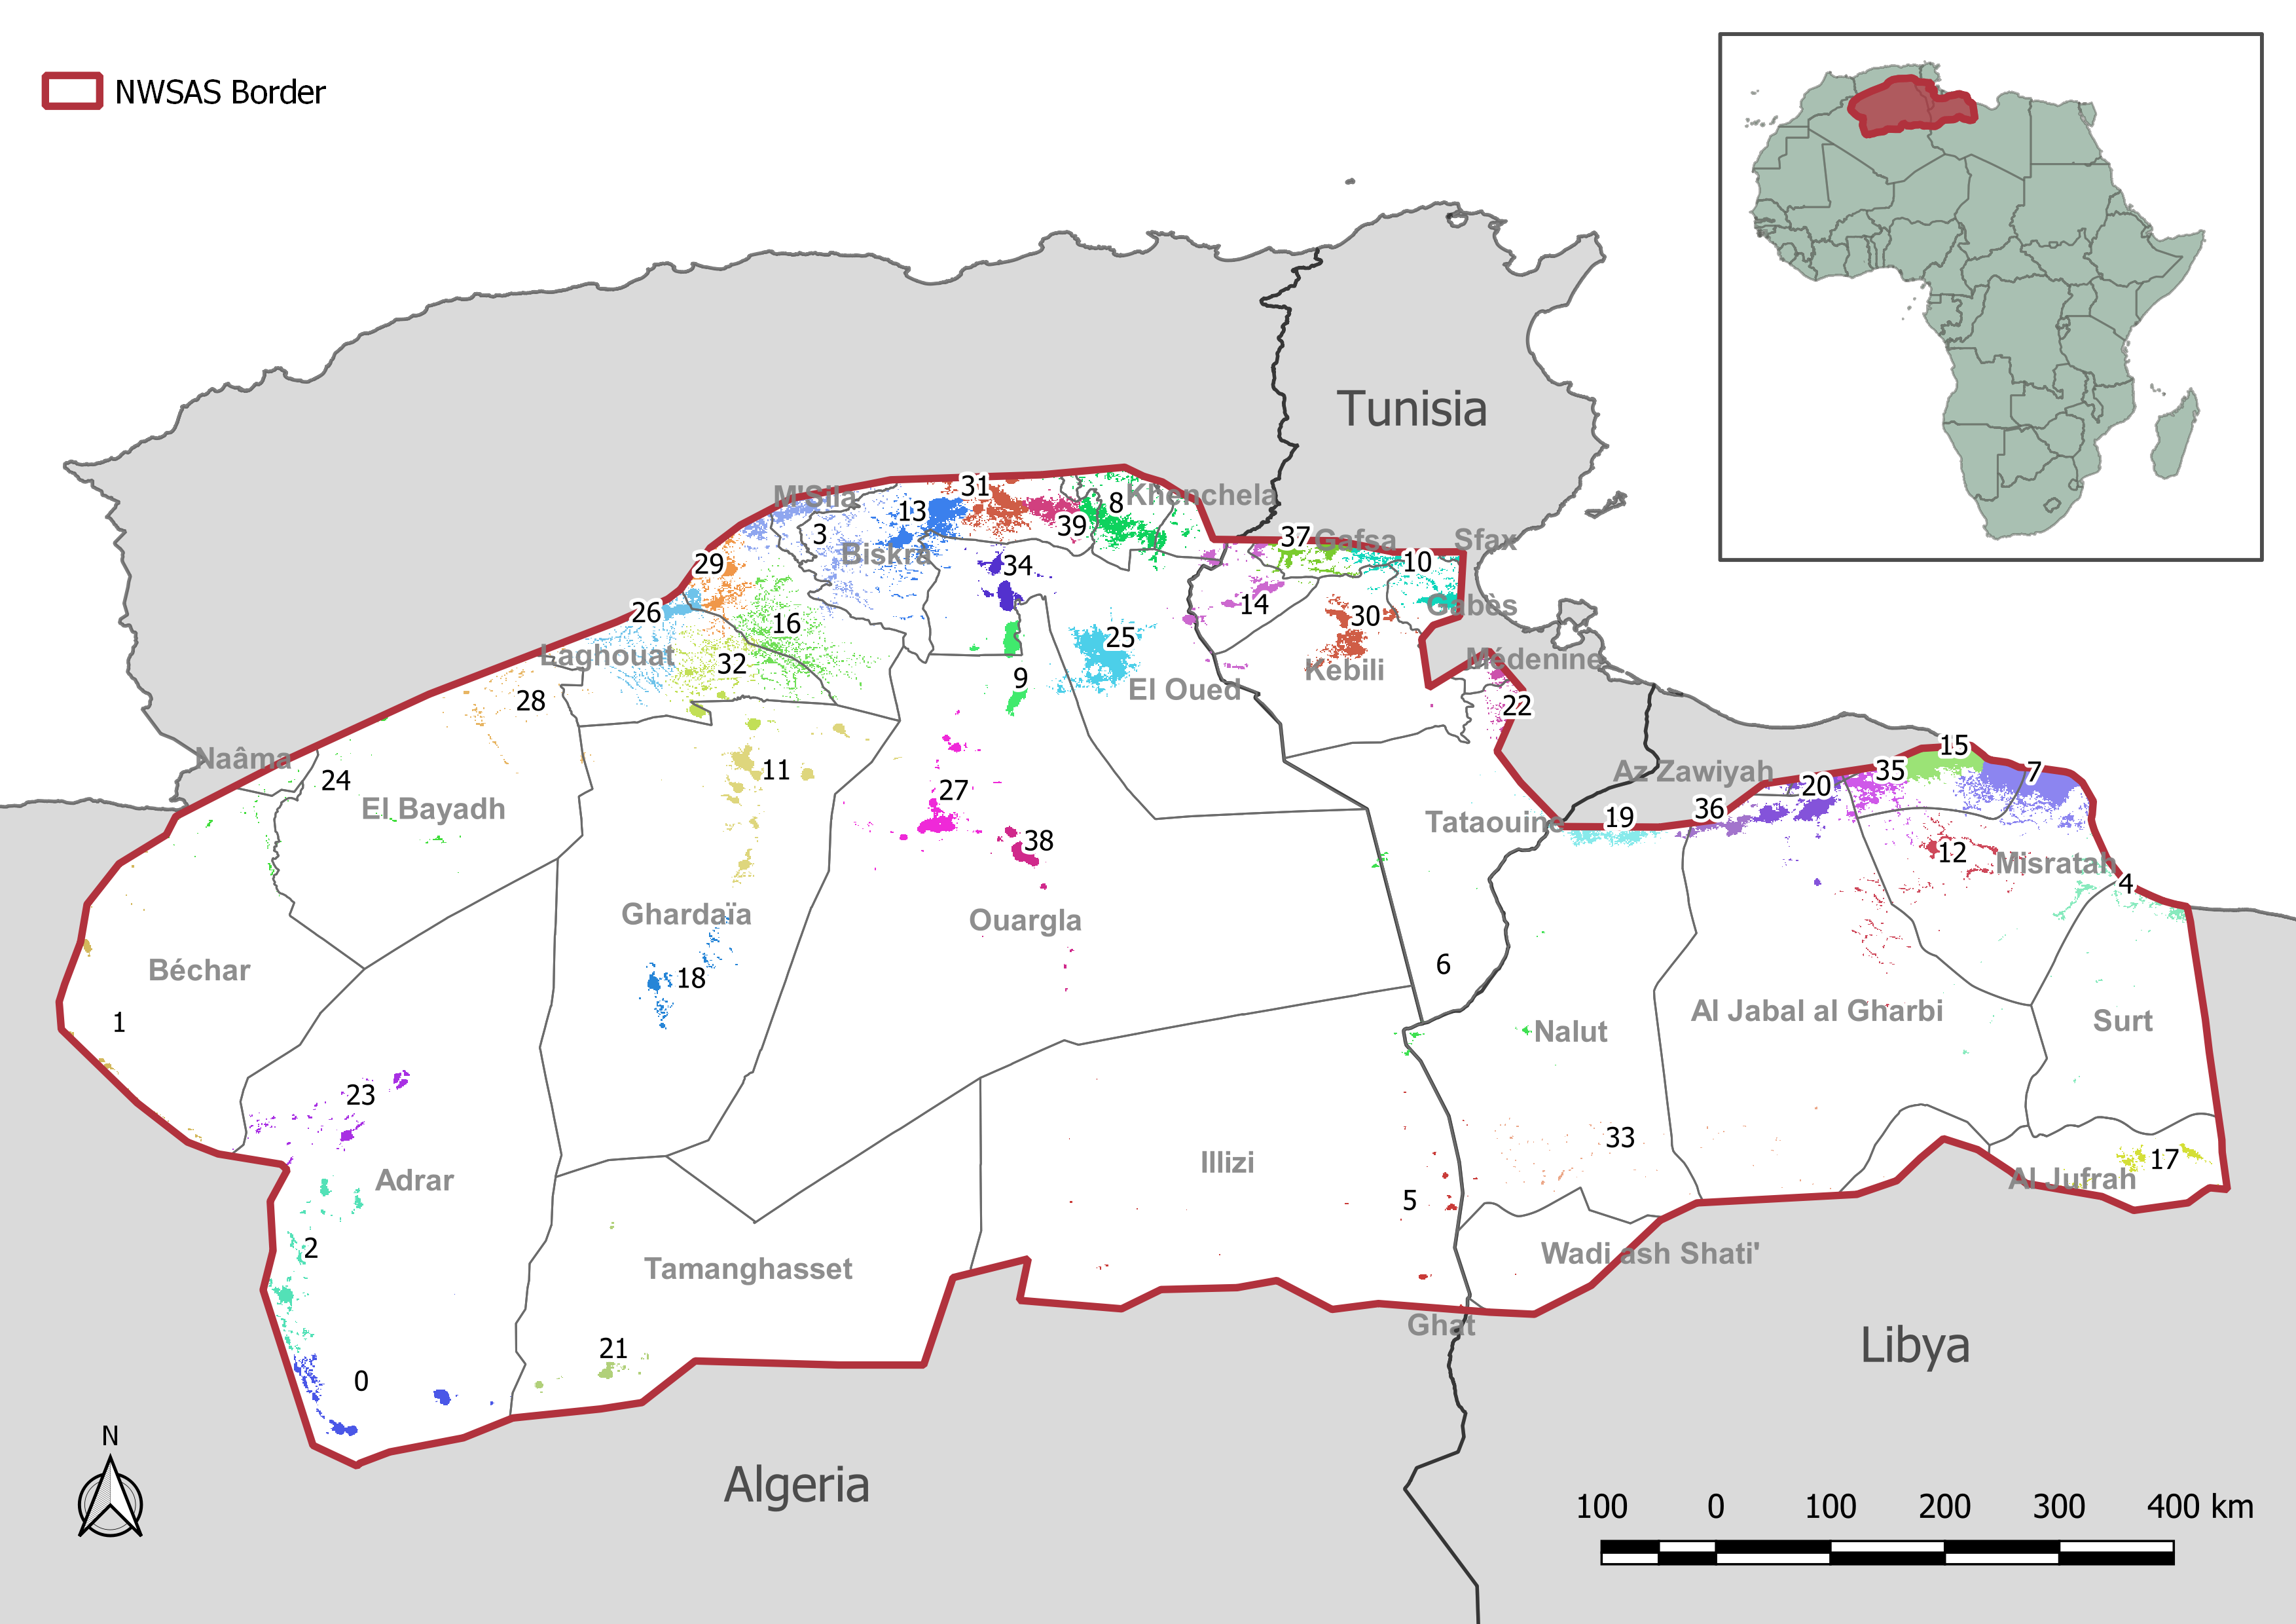
\includegraphics[width=0.88\textwidth, cfbox=black 1pt 0pt]{NWSAS_clusters}
	\caption{Population and cropland clusters.}
	\label{fig:clusters}
\end{figure} 

Clusters are numbered from 0 to 39, yielding 40 agglomerations including each population and cropland areas. Every cluster is tagged with a number and colored to make them stand out from others.


\section{Water extractions and reuse per cluster}
Figure \autoref{fig:BaselineWater} shows the water extractions for agricultural irrigation and population consumption per cluster fo the Baseline scenario. 

Cluster 7 represents by far, the largest amount of water extractions, this cluster is a combination of population and agricultural irrigation areas from the Al Marqab and Misratah provinces in Libya. It is followed by cluster 8 comprising mainly agricultural irrigation areas of the Khenchela province in Algeria. Then follows cluster 13 and 25 from the northern part of Algerian portion of the basin and cluster 15 of the Al Marqab province in Libya.

All points inside the Biskra province are subdivided into clusters number 13, 31, 39 and 3, which combined represent the major water extractions of the region. However when analysed individually, their impact is reduced, being cluster 13 the most representative.

Overall, Algeria accounts for most of the water extractions, comprising clusters 8, 13, 25, 31, 3 and 26, which rank inside the 10 highest water consumers. 

The activity of Tunisia inside the basin is low in comparison with the other two countries. The most representative cluster is number 30 in Kebili, ranking 6 in water extractions.

\newpage
\begin{figure}[!h]
	\centering
	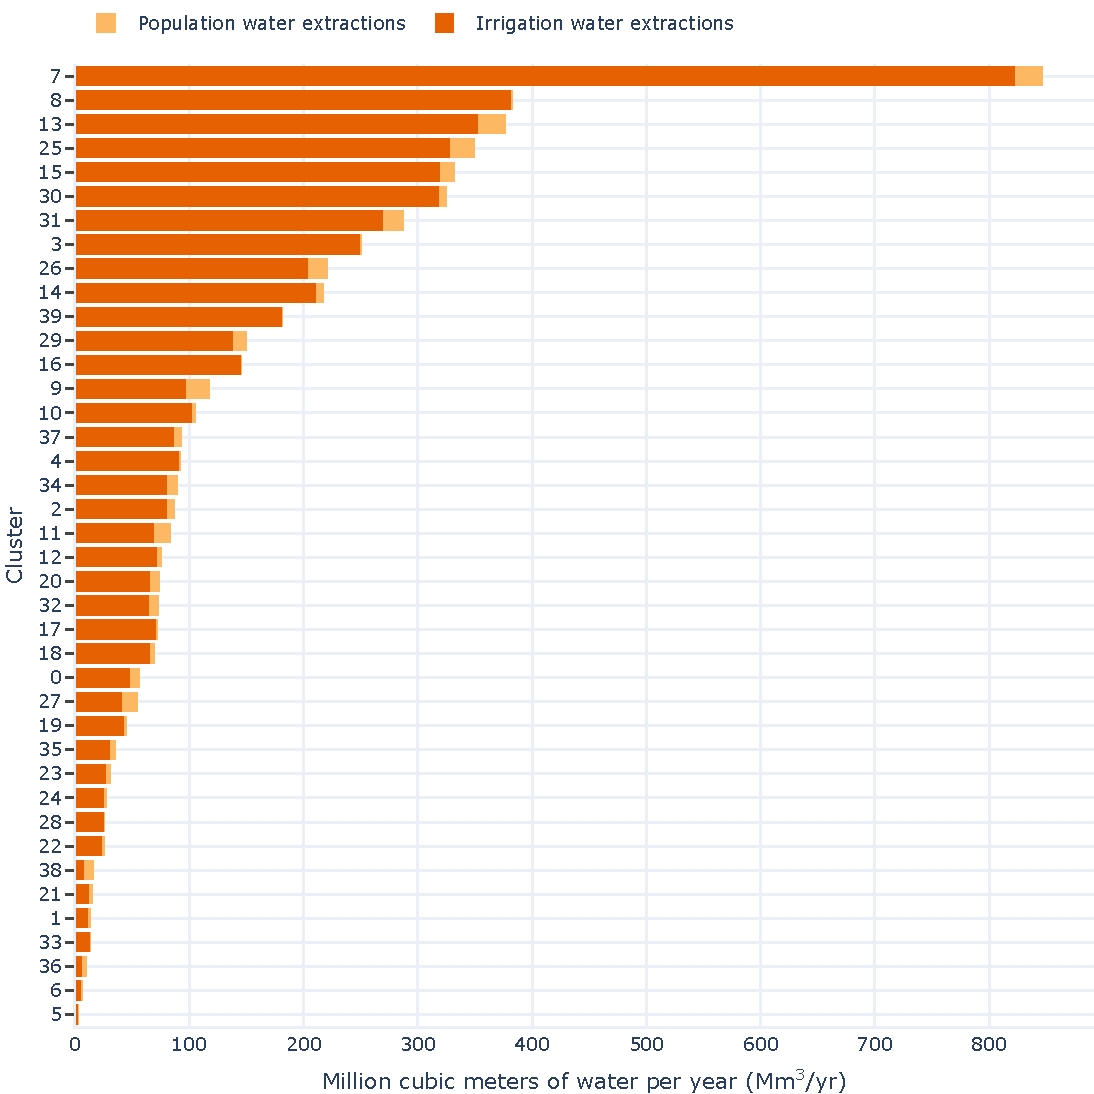
\includegraphics[width=\textwidth]{BaselineWater2}
	\caption{Water extractions by cluster. Baseline scenario.}
	\label{fig:BaselineWater}
\end{figure}\newpage

In figure \autoref{fig:SubAgLowPopWater} the extractions per sector and treated wastewater reused by source is shown for each cluster for the Subsidized agricultural water and low population water scenario. The clusters, are organized from high to low value of total water extractions.

Again, cluster 7 represents the largest amount of water extractions. It is followed by clusters 15, 8, 25 and 13. It is interesting to notice that the rankings of those clusters in the overall water extractions, changed from the Baseline to the subsidized scenario with water reuse.

\begin{figure}[!h]
	\centering
	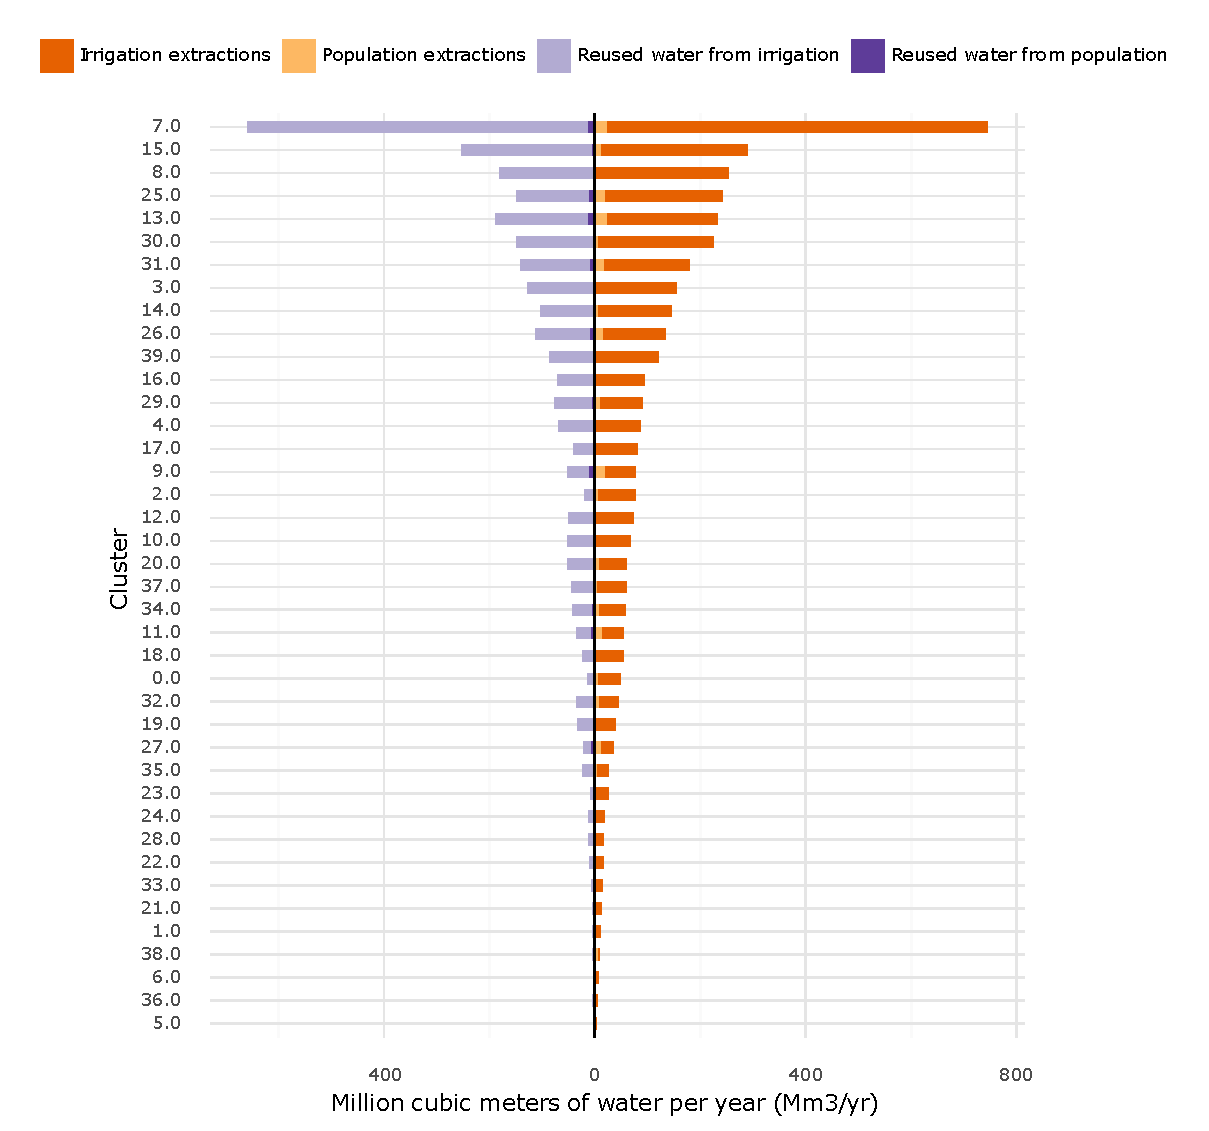
\includegraphics[width=\textwidth]{Sub_agri_water_Low_pop_water}
	\caption{Water extractions and reuse by cluster. Subsidized agricultural water extractions and low population water demand scenario. At left: reused water after reclaim, treatment and allocation classified by population and irrigation source. At right: overall water extractions classified by population and irrigation use.}
	\label{fig:SubAgLowPopWater}
\end{figure}
\newpage

Figure \autoref{fig:SubAgHighPopWater} shows water extractions for the Subsidized agricultural water and high population water scenario. It presents an almost exact behaviour as the previous case, with slightly higher extractions due to the higher population demand and some clusters swaping places in the low ends as clusters 38 and 1.

\begin{figure}[!h]
	\centering
	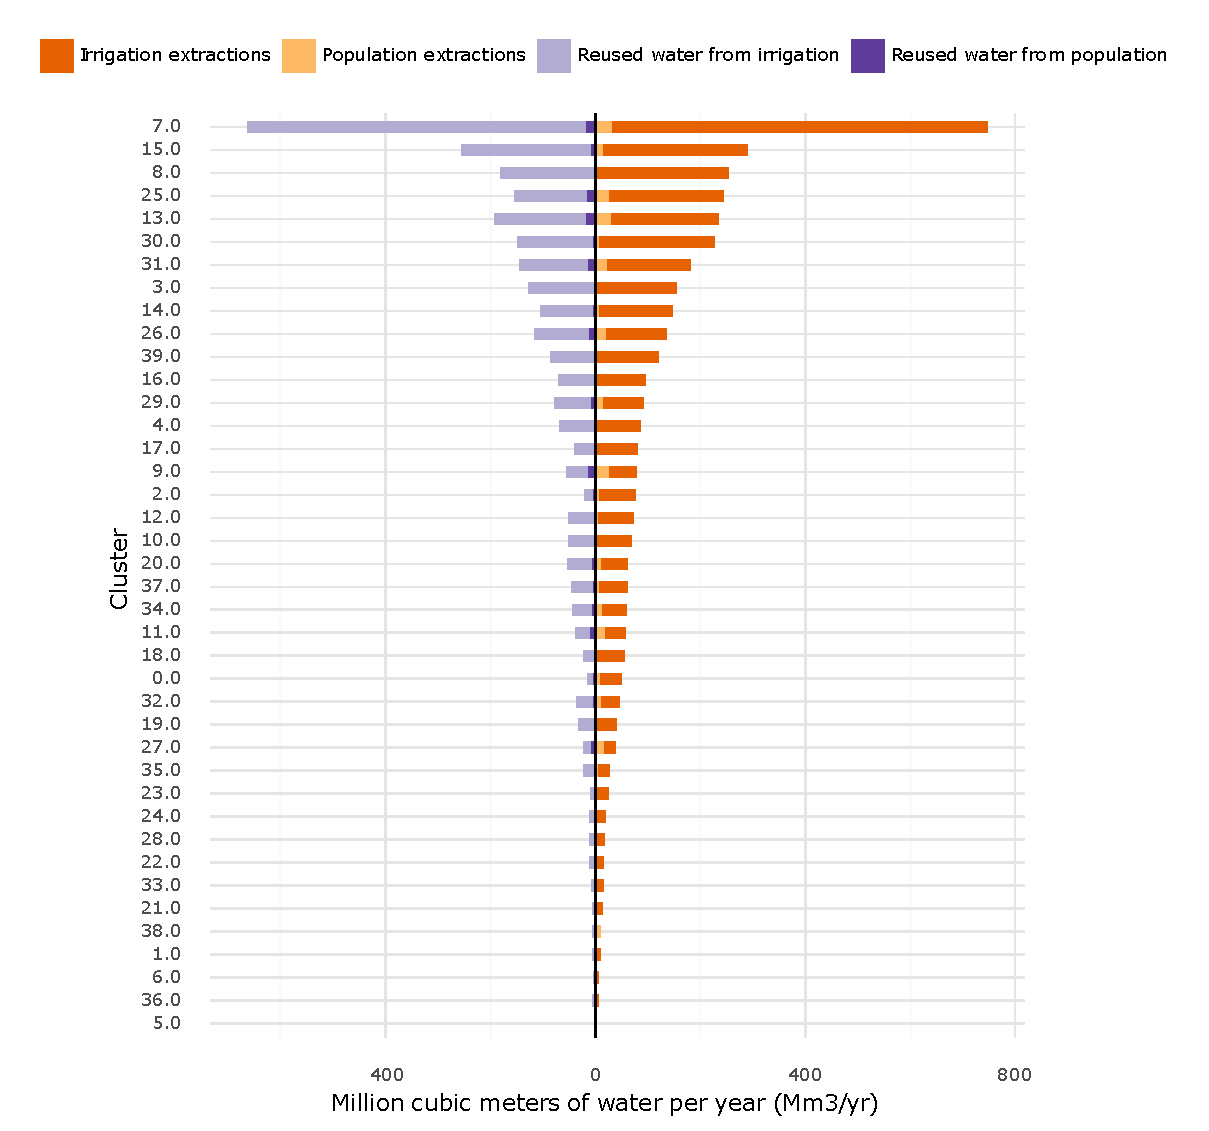
\includegraphics[width=\textwidth]{Sub_agri_water_High_pop_water}
	\caption{Water extractions and reuse by cluster. Subsidized agricultural water extractions and high population water demand scenario. At left: reused water after reclaim, treatment and allocation classified by population and irrigation source. At right: overall water extractions classified by population and irrigation use.}
	\label{fig:SubAgHighPopWater}
\end{figure}
\newpage

Figure \autoref{fig:FreeAgLowPopWater} shows water extractions for the free agricultural water and low population water scenario. It presents an almost exact behaviour as the subsidez case, but with higher extractions due to the lower agricultural water demand. Again some clusters swaped places as clusters 13 and 25.

\begin{figure}[!h]
	\centering
	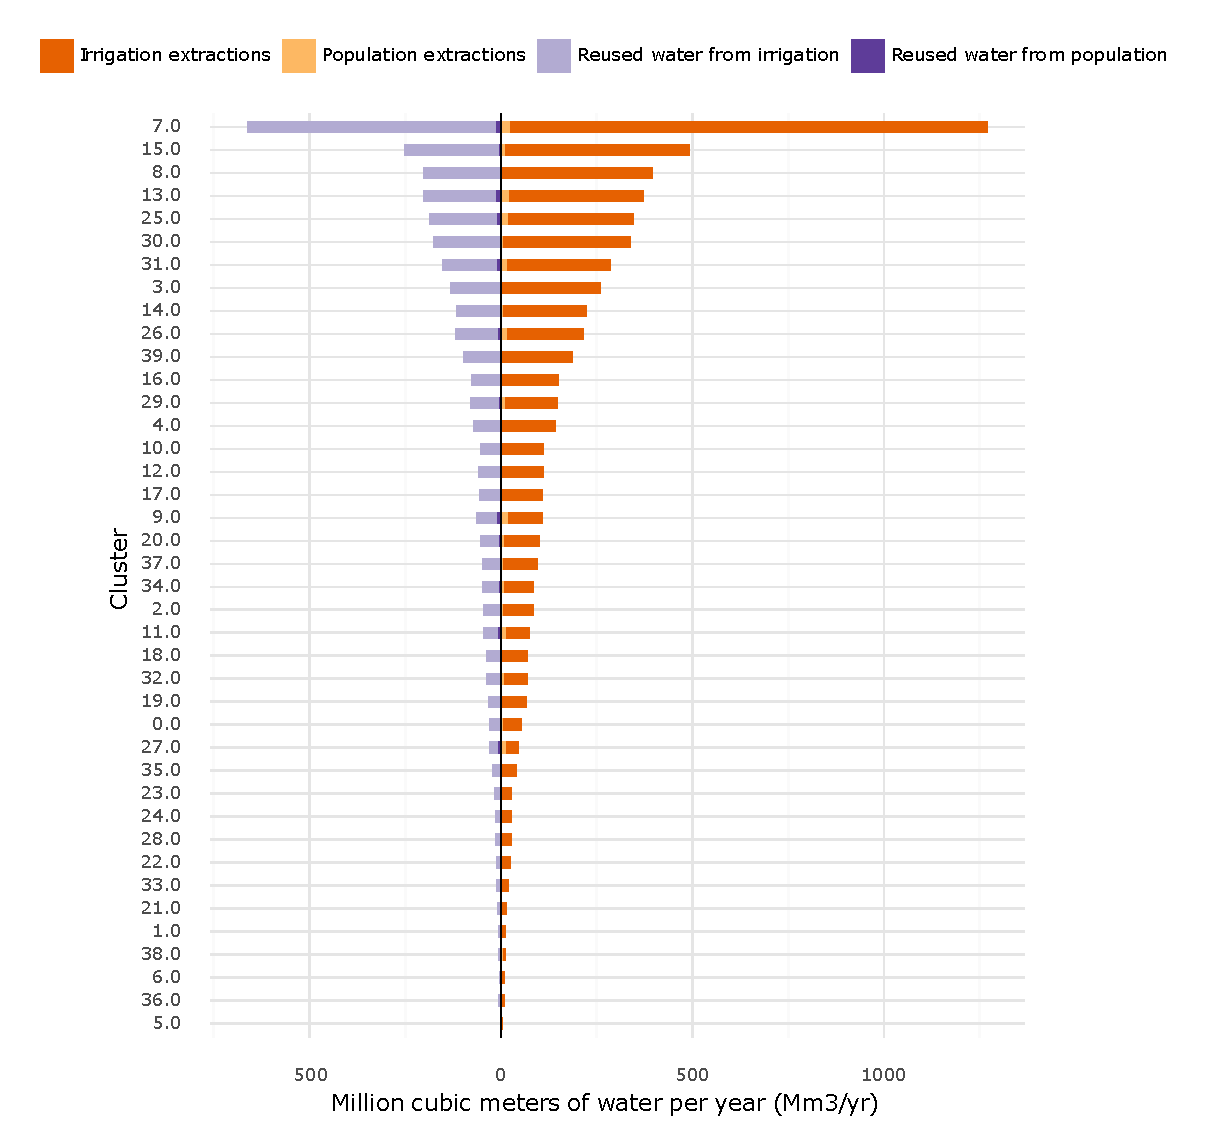
\includegraphics[width=\textwidth]{Free_agri_water_Low_pop_water}
	\caption{Water extractions and reuse by cluster. Free agricultural water extractions and low population water demand scenario. At left: reused water after reclaim, treatment and allocation classified by population and irrigation source. At right: overall water extractions classified by population and irrigation use.}
	\label{fig:FreeAgLowPopWater}
\end{figure}
\newpage

Figure \autoref{fig:FreeAgHighPopWater} shows water extractions for the free agricultural water and high population water scenario. It presents an almost exact behaviour as the previous case, but with slightly higher extractions due to the higher population demand.

\begin{figure}[!h]
	\centering
	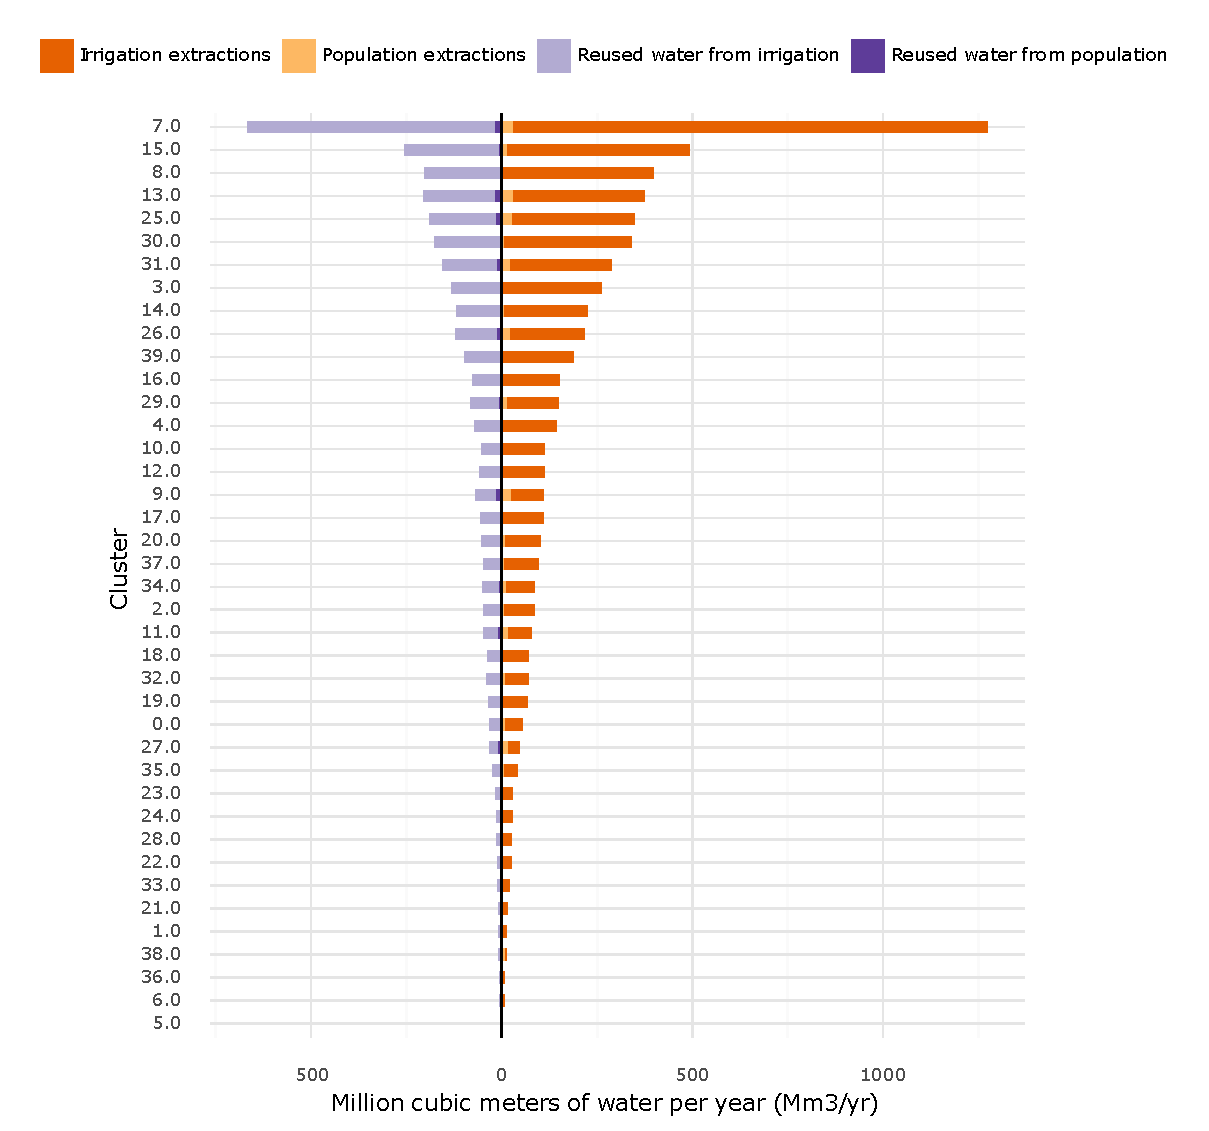
\includegraphics[width=\textwidth]{Free_agri_water_High_pop_water}
	\caption{Water extractions and reuse by cluster. Free agricultural water extractions and high population water demand scenario. At left: reused water after reclaim, treatment and allocation classified by population and irrigation source. At right: overall water extractions classified by population and irrigation use.}
	\label{fig:FreeAgHighPopWater}
\end{figure}
\newpage

Finally, water extraction for the private agricutural regime and low to high population water demand, are presented in figures \ref{fig:PrivAgLowPopWater} and \ref{fig:PrivAgHighPopWater} respectively. Water extractions are much lower in this scenario compared to the free agricultural water scenarios, however the diferences are not that high with the subsidized ones. This is due to the higher amount of available water for reuse in the subsidized scenarios, which can be seen in the left part of the graphs. Furthermore, the clusters rankings were the same as for the subsidezed cases.

\begin{figure}[!h]
	\centering
	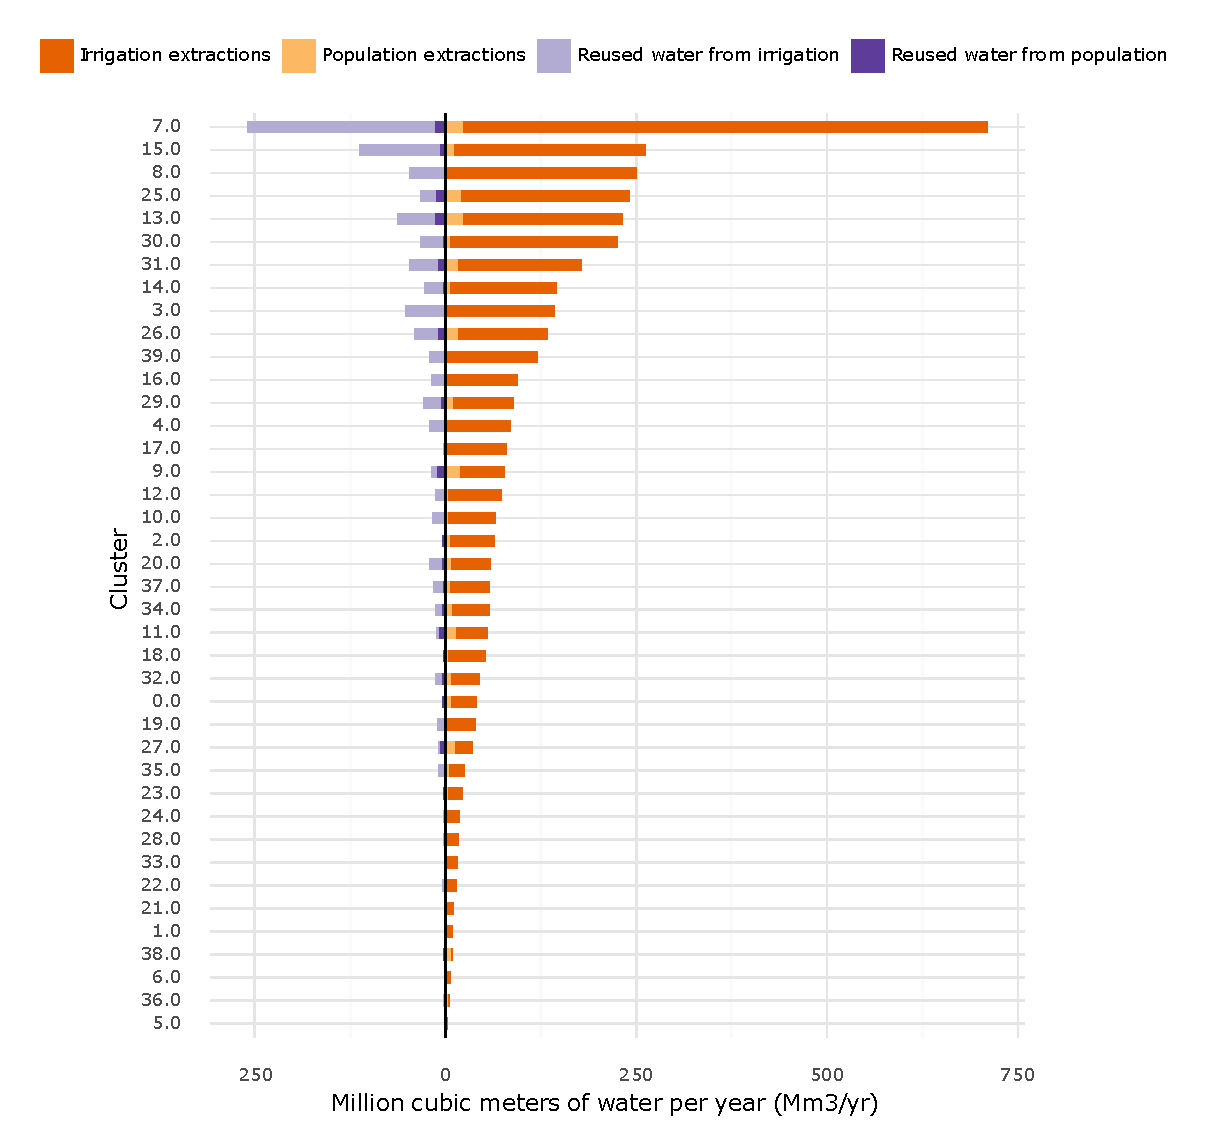
\includegraphics[width=\textwidth]{Priv_agri_water_Low_pop_water}
	\caption{Water extractions and reuse by cluster. Private agricultural water extractions and low population water demand scenario. At left: reused water after reclaim, treatment and allocation classified by population and irrigation source. At right: overall water extractions classified by population and irrigation use.}
	\label{fig:PrivAgLowPopWater}
\end{figure}
\newpage

\begin{figure}[!h]
	\centering
	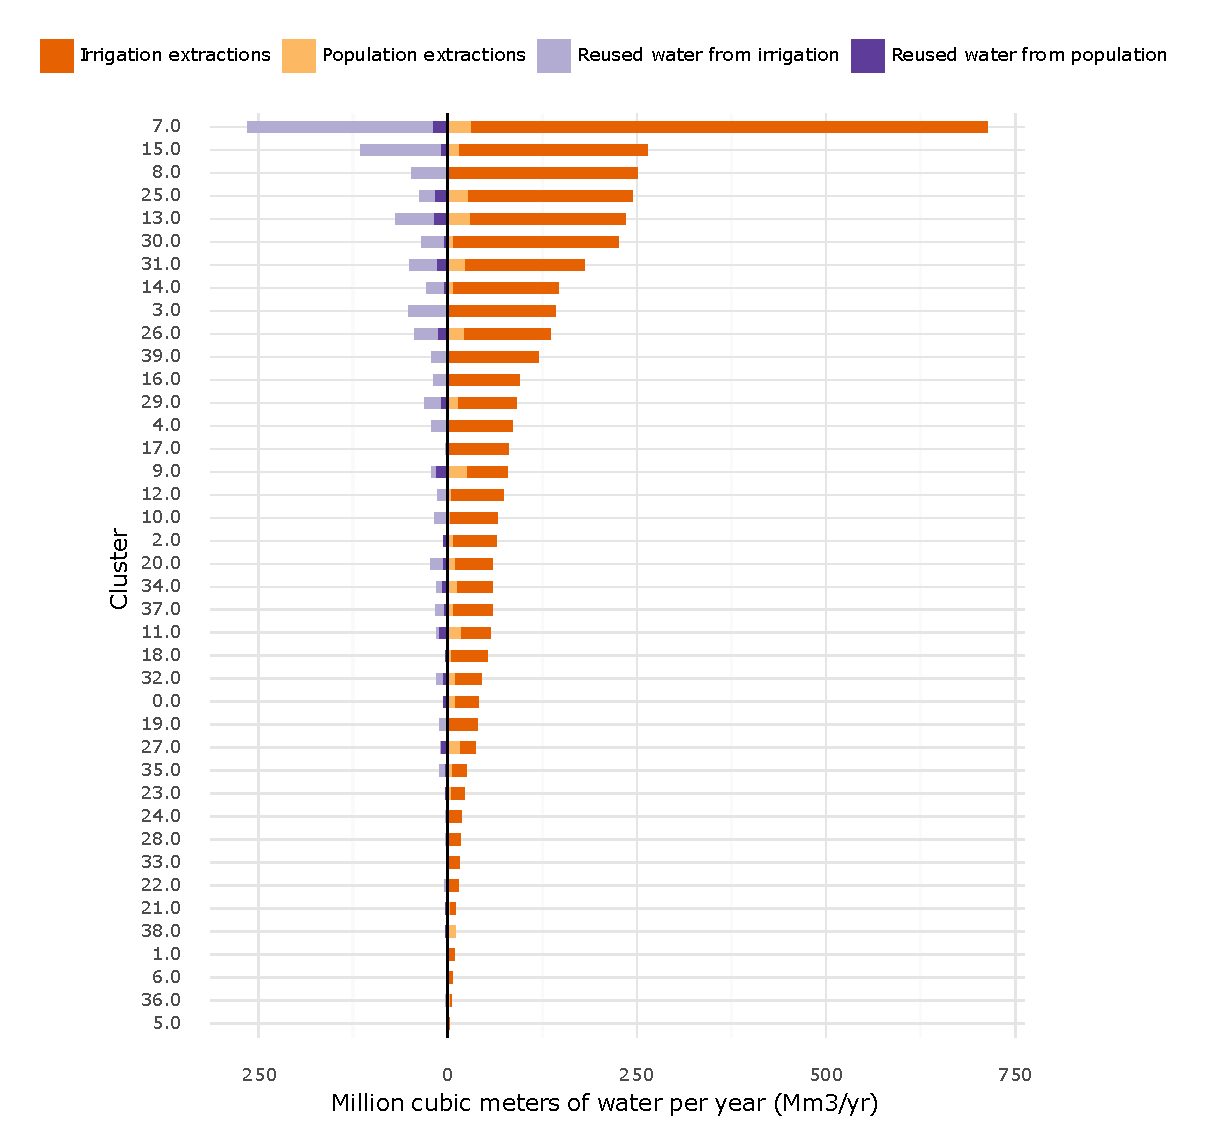
\includegraphics[width=\textwidth]{Priv_agri_water_High_pop_water}
	\caption{Water extractions and reuse by cluster. Private agricultural water extractions and high population water demand scenario. At left: reused water after reclaim, treatment and allocation classified by population and irrigation source. At right: overall water extractions classified by population and irrigation use.}
	\label{fig:PrivAgHighPopWater}
\end{figure} 
\newpage

\section{Energy demand per cluster}
In this section, additional results concerning the energy requirements for water pumping, water desalination and wastewater treatment are presented.
\begin{figure}[!h]
	\centering
	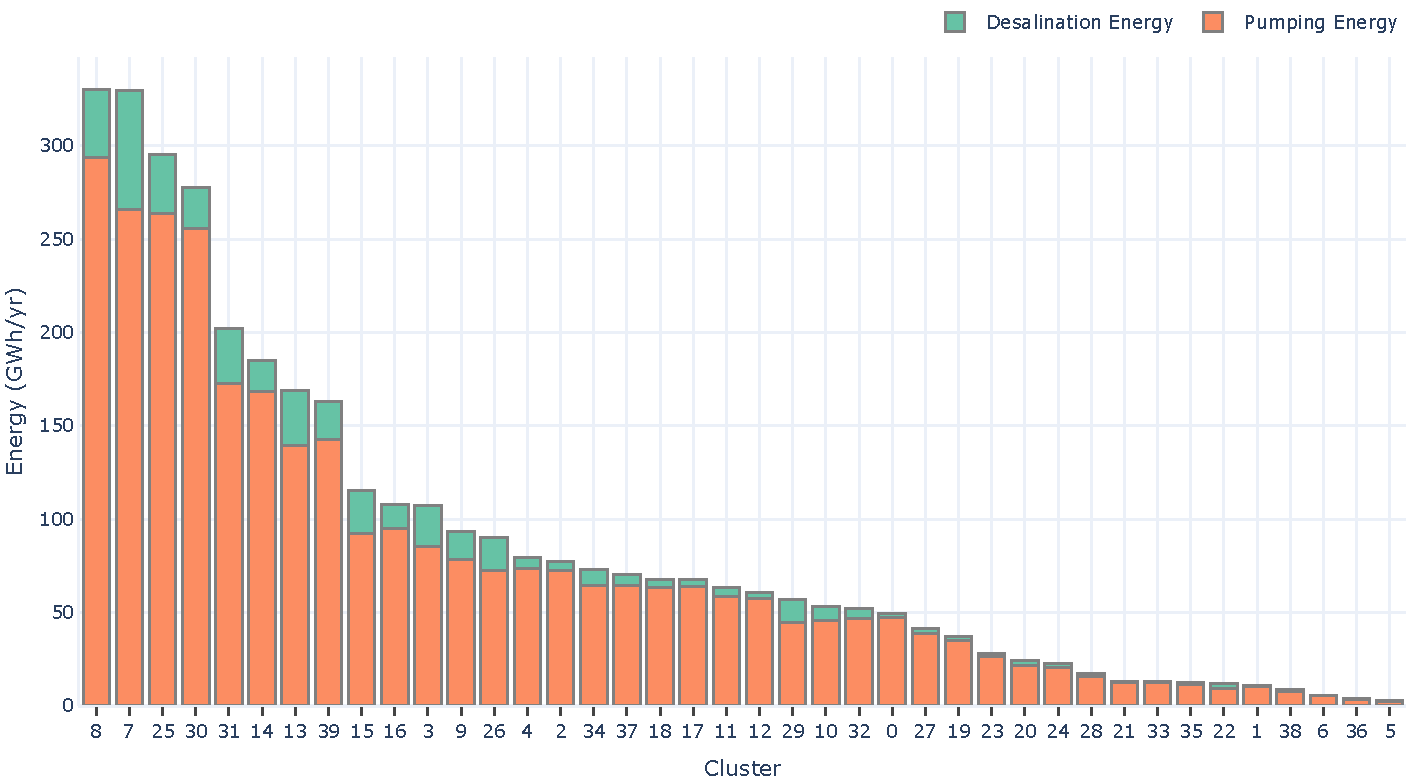
\includegraphics[width=\textwidth]{BaselineEnergyPerCluster}
	\caption{Annual energy demand by cluster in the Baseline scenario.}
	\label{fig:BaselineEnergyPerCluster}
\end{figure} 

\begin{figure}[!h]
	\centering
	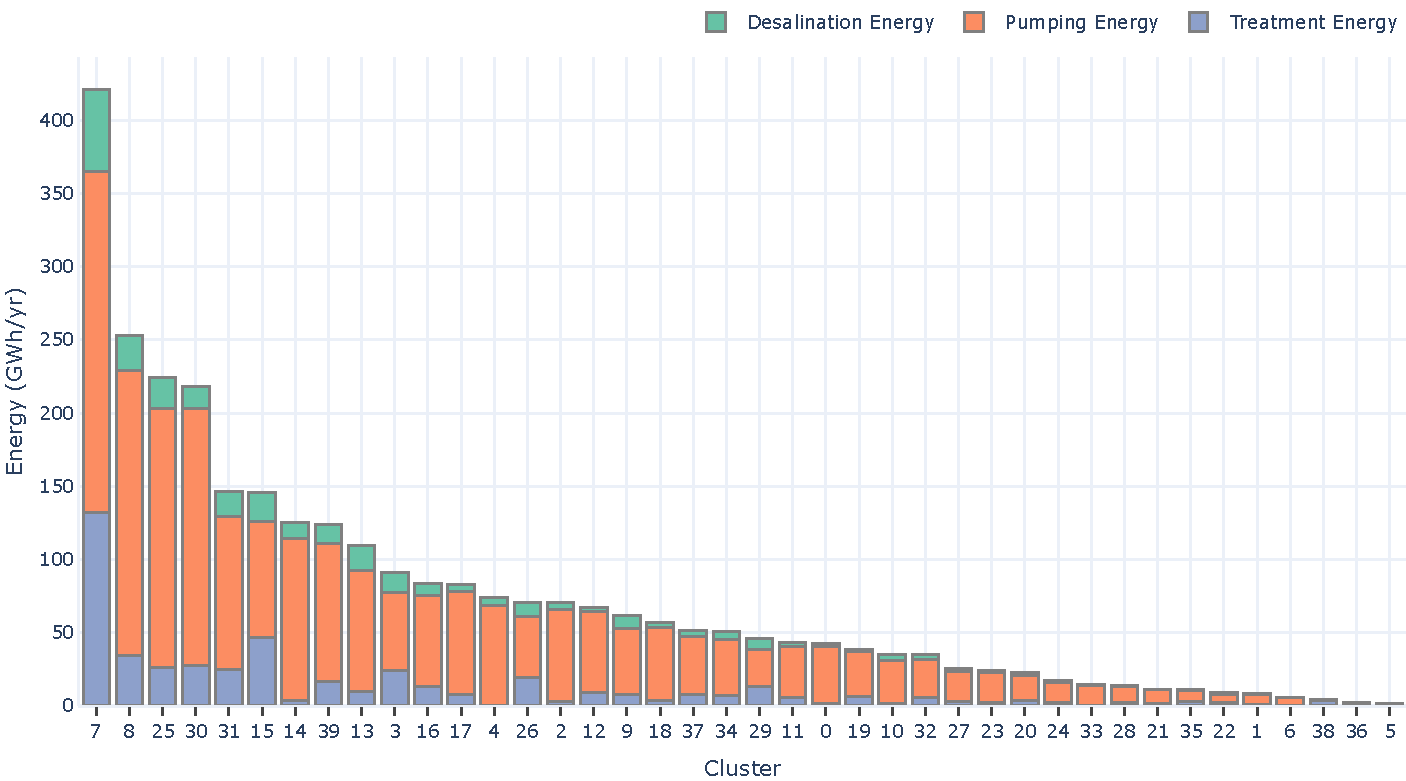
\includegraphics[width=\textwidth]{SubAgLowPopEnergyPerCluster}
	\caption{Annual energy demand by cluster in the subsidized agricultural water and low population water scenario.}
	\label{fig:SubAgLowPopEnergyPerCluster}
\end{figure}\newpage

\begin{figure}[!h]
	\centering
	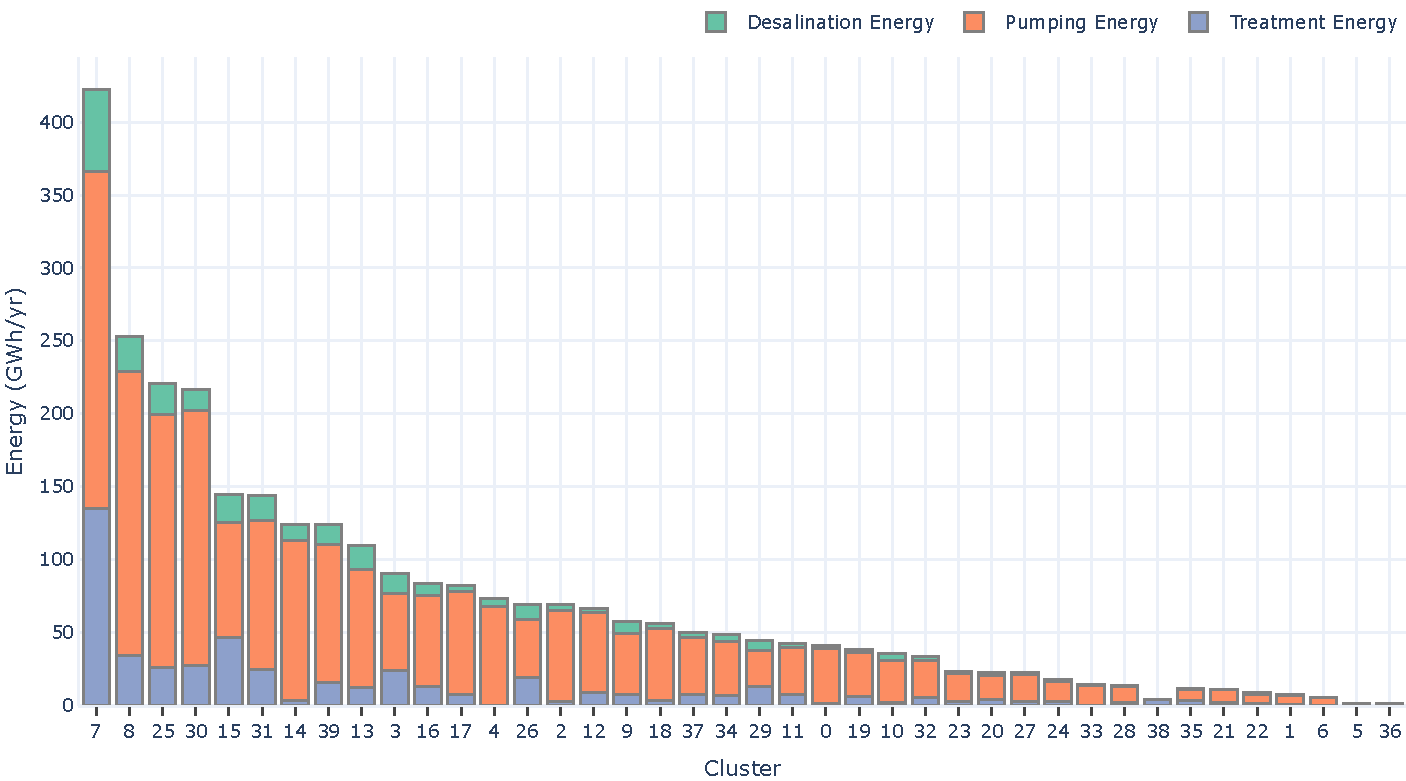
\includegraphics[width=\textwidth]{SubAgHighPopEnergyPerCluster}
	\caption{Annual energy demand by cluster in the subsidized agricultural water and high population water scenario.}
	\label{fig:SubAgHighPopEnergyPerCluster}
\end{figure} 

\begin{figure}[!h]
	\centering
	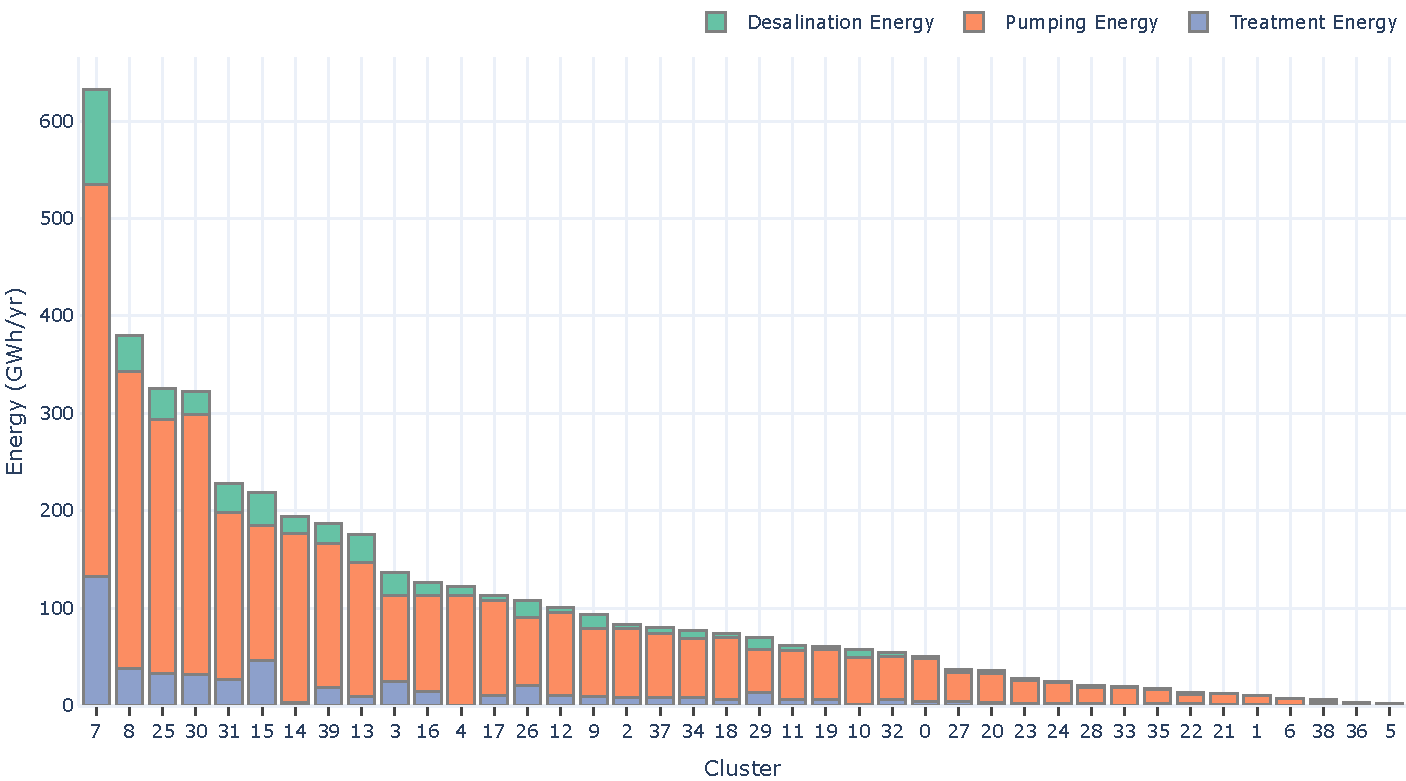
\includegraphics[width=\textwidth]{FreeAgLowPopEnergyPerCluster}
	\caption{Annual energy demand by cluster in the free agricultural water and low population water scenario.}
	\label{fig:FreeAgLowPopEnergyPerCluster}
\end{figure}\newpage

\begin{figure}[!h]
	\centering
	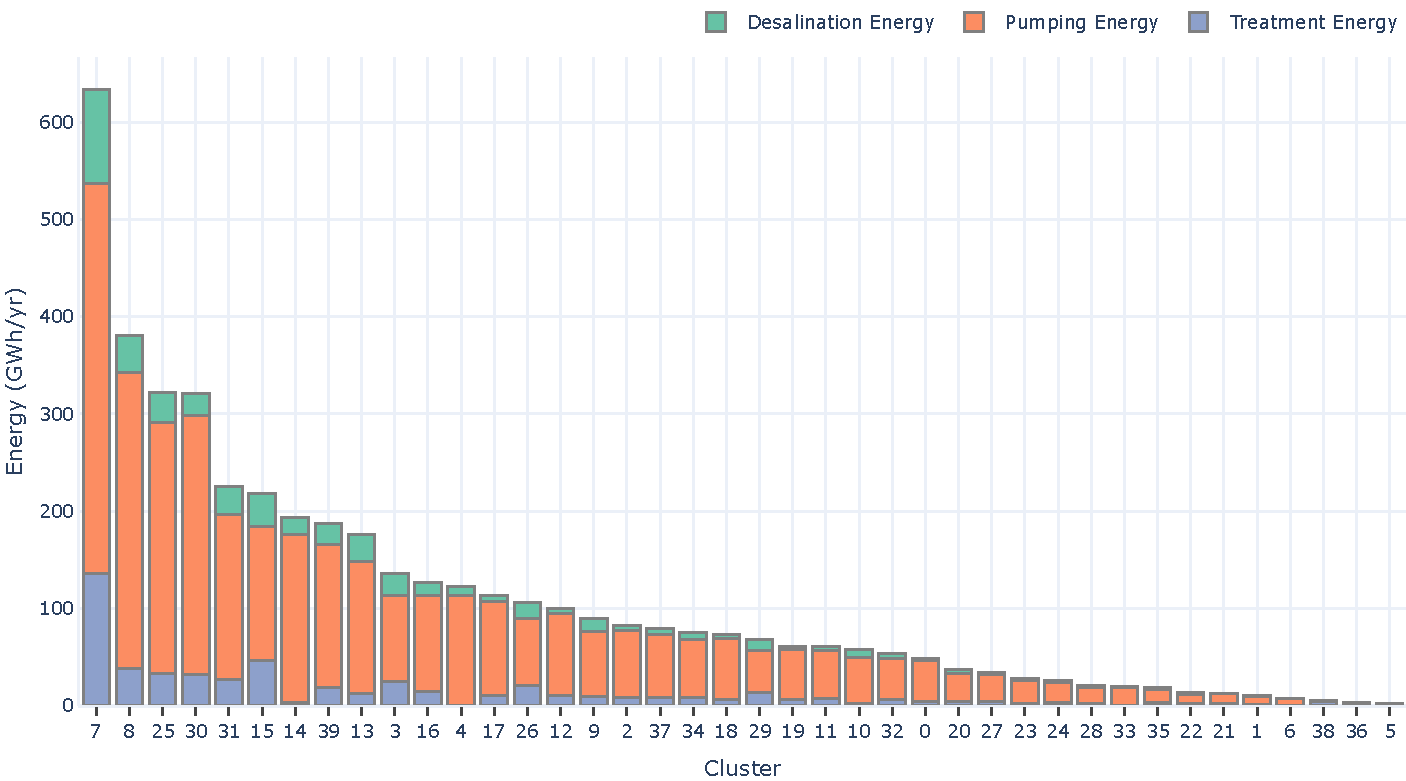
\includegraphics[width=\textwidth]{FreeAgHighPopEnergyPerCluster}
	\caption{Annual energy demand by cluster in the free agricultural water and high population water scenario.}
	\label{fig:FreeAgHighPopEnergyPerCluster}
\end{figure}

\begin{figure}[!h]
	\centering
	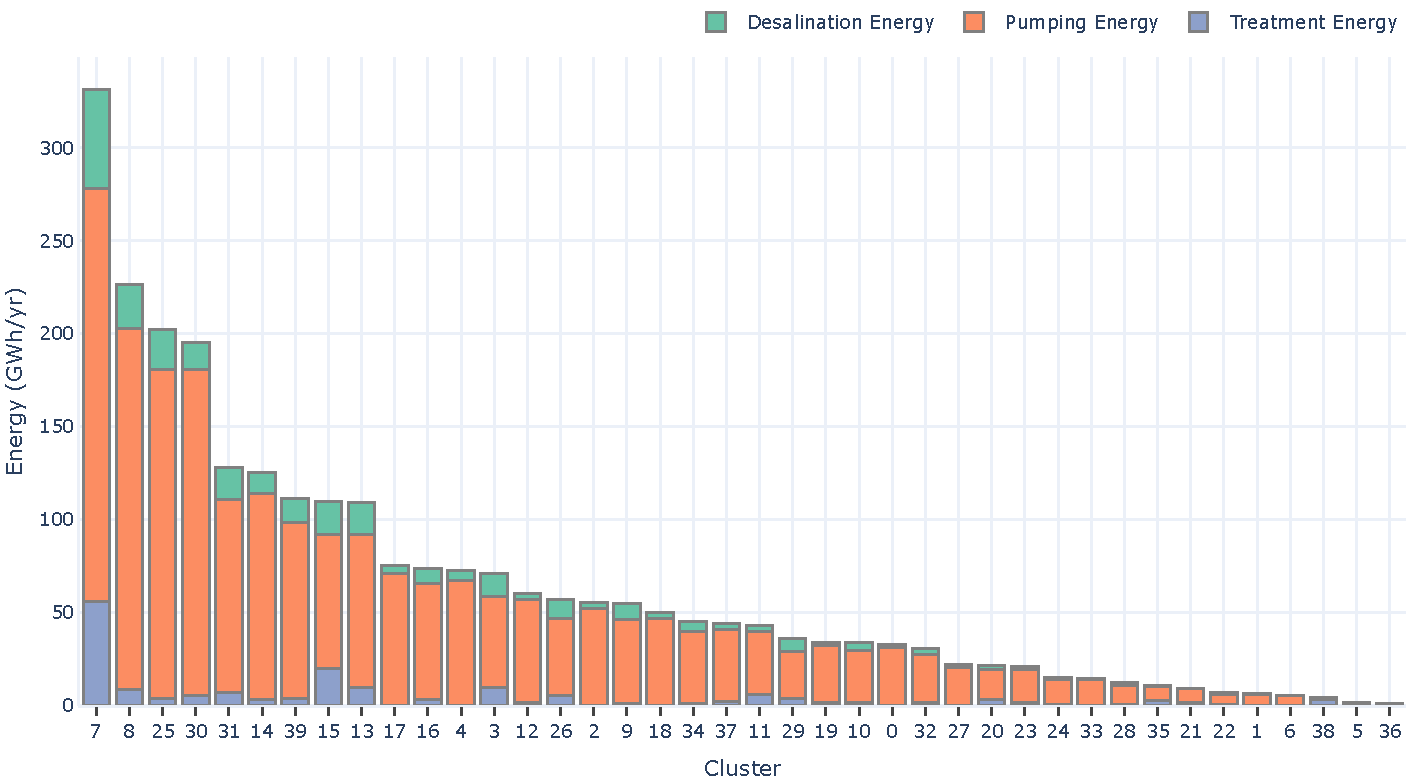
\includegraphics[width=\textwidth]{PrivAgLowPopEnergyPerCluster}
	\caption{Annual energy demand by cluster in the private agricultural water and low population water scenario.}
	\label{fig:PrivAgLowPopEnergyPerCluster}
\end{figure}\newpage

\begin{figure}[!h]
	\centering
	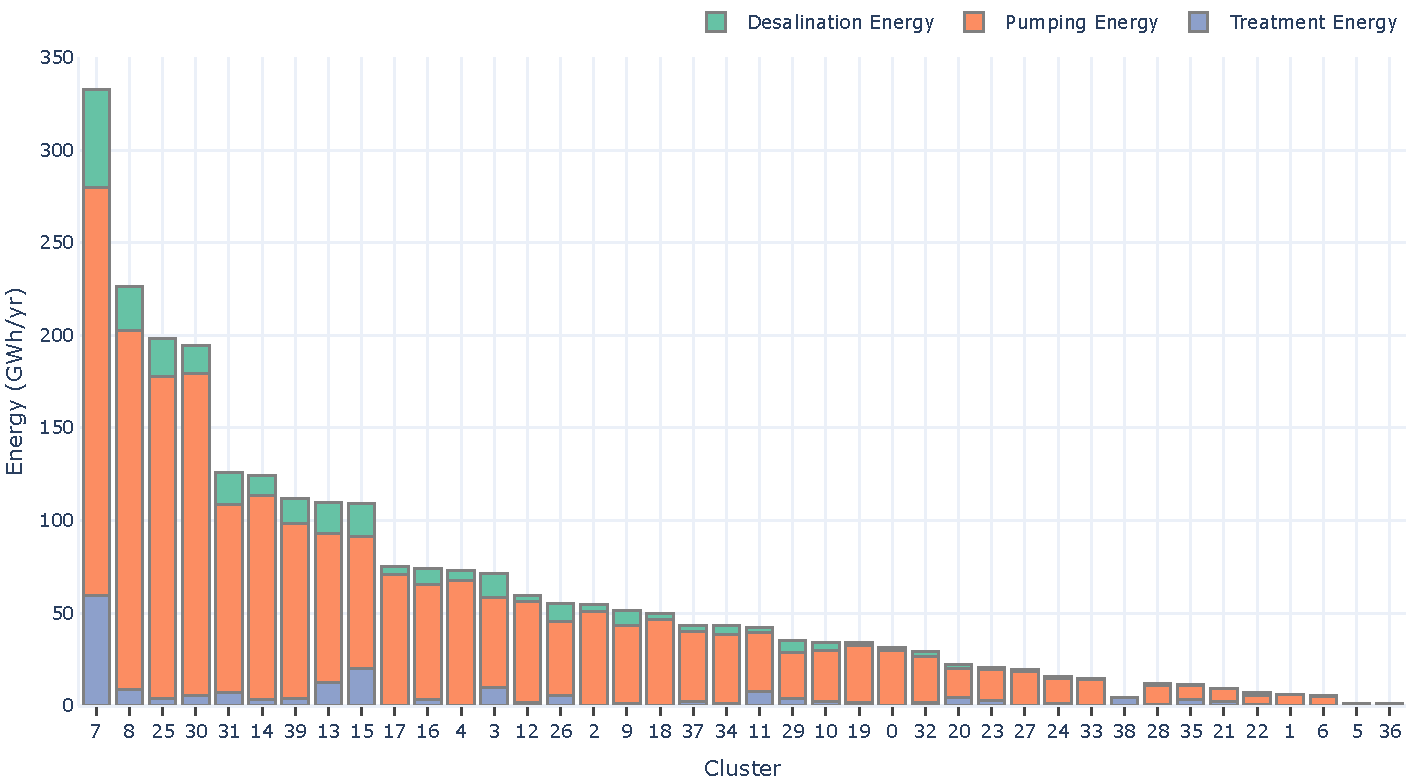
\includegraphics[width=\textwidth]{PrivAgHighPopEnergyPerCluster}
	\caption{Annual energy demand by cluster in the private agricultural water and high population water scenario.}
	\label{fig:PrivAgHighPopEnergyPerCluster}
\end{figure}


\newcommand{\newblock}{}
\bibliography{References}
\bibliographystyle{unsrtnat}

\end{document}